\documentclass[12pt]{article}

%%% All setup/preamble moved to a different file
%%% from Anna
\usepackage{ifthen,pifont,latexsym}
\usepackage[T1]{fontenc}
\usepackage{times,avant}
\usepackage{comment}
\usepackage{datetime}

%%\usepackage{mathrsfs}
%\usepackage[mtpluscal,mtplusscr,T1]{mathtime}
\usepackage[round,authoryear]{natbib}
%%
\usepackage[pdftex]{graphicx}
%%
\def\Includefigs{true}
%%\usepackage{amsmath}
%%
%% \usepackage{draftmark}\markdraftpage
%%
%%%%%%%%%% Other preamble commands here ...
%%
%%
\def\rfeqn#1{(\ref{eq.#1})}
\def\vs#1{\vspace{#1\baselineskip}}
\def\HeadSpace{\vs{.17}}
\def\BoldHead#1{\HeadSpace\textbf{#1}}
\def\ItalHead#1{\HeadSpace\textit{#1}}
\def\UlHead#1{\HeadSpace\underline{#1}}
\def\floatpagefraction{.7}
%%
\newenvironment{descz}{\begin{description}\def\itemsep{0in}}%%
{\end{description}}
\newenvironment{itemz}{\begin{itemize}\def\itemsep{0in}}%%
{\end{itemize}}
\newenvironment{enumz}{\begin{enumerate}\def\itemsep{0in}}%%
{\end{enumerate}}
\newcommand{\m}{\ensuremath{\mathbf{\mu}}}
\newcommand{\s}{\ensuremath{\mathbf{\Sigma}}}
\newcommand{\bx}{\textbf{x}}


%%\input acronyms.tex
%%
%% Def's and macros
%%
% \mathscr changed to \mathcal in the following by APS
\def\DB{\ensuremath{\mathbf{D}}} %% Database
\def\QS{\ensuremath{\mathscr{Q}}} %% Query space
\def\DR{\ensuremath{\mathbf{DR}}} %% Disclosure risk
\def\DU{\ensuremath{\mathbf{DU}}} %% Data utility
\def\DD{\ensuremath{\mathbf{DD}}} %% Data distortion
\def\RS{\ensuremath{\mathbf{R}}} %% Release space
\def\DBORIG{\ensuremath{{D}_{\mathrm{orig}}}} %% Database
\def\DBPOST{\ensuremath{\mathscr{D}_{\mathrm{post}}}} %% Database
\def\DBREL{\ensuremath{D_{\mathrm{rel}}}} %% Released database
%% Methods
\def\NOI{{\tt Noise}}
\def\MICZ{{\tt Micz}}
\def\MICP{{\tt Micp}}
\def\MICM{{\tt Micm_all}}
\def\MICI{{\tt Micir}}
\def\MIC7{{\tt Micm_groups}}
\def\RESAMP{{\tt Resamp}}
\def\RANK{{\tt Rank}}
%% Utility measures
\def\LR{\ensuremath{\mathbf{LR}}} %% Likelihood ratio
\def\KL{\ensuremath{\mathbf{KL}}} %% KL measure
\def\IO{\ensuremath{\mathbf{IO}}} %% interval overlap measure
\def\EO{\ensuremath{\mathbf{EO}}} %% ellipsoid overlap measure
%\def\argmax{\operatornamewithlimits{arg\max}}
\def\SDL{statistical disclosure limitation (SDL)%%
    \gdef\SDL{SDL}}
    
%%%%%% END ANNA CONFIG

\usepackage{hyperref}


\begin{comment}
Place \usepackage{glossaries} and \makeglossaries in your preamble
(after \usepackage{hyperref} if present). Then define any number of
\newglossaryentry and \newacronym glossary and acronym entries in your
preamble (recommended) or before first use in your document
proper. Finally add a \printglossaries call to locate the glossaries
list within your document structure. Then pepper your writing with
\gls{mylabel} macros (and similar) to simultaneously insert your
predefined text and build the associated glossary. File processing
must now include a call to makeglossaries followed by at least one
further invocation of latex or pdflatex -
https://en.wikibooks.org/wiki/LaTeX/Glossary
\end{comment}
\usepackage[toc, nonumberlist, nopostdot, xindy]{glossaries}
\usepackage{glossaries-extra}
\glssetcategoryattribute{general}{glossname}{title}

\makeglossaries
% Note: This package is fragile and you need to use \\ between
% paragraphs in a multi-paragraph description
%
\newglossaryentry{sensitivity}{
    name=sensitivity,
    description={When referring to \gls{differential_privacy}, the US Census
    Bureau uses the term \emph{sensitivity} to denote the impact that
    a single person can have on the computation of a statistic. In the
    \gls{differential_privacy} literature this quantity is properly referred
    to as the $l_1$ sensitivity.\\
    \\
     ``The $l_1$ sensitivity of a function $f$ captures the
    magnitude by which a single individual’s data can change the
    function $f$ in the worst case, and therefore, intuitively, the
    uncertainty in the response that we must introduce in order to
    hide the participation of a single individual.'' \parencite{dwork_algorithmic_2013} \\
    \\
    ``The sensitivity of a counting query is 1 (the
    addition or deletion of a single individual can change a count by
    at most 1)'' \parencite{dwork_algorithmic_2013} }
}

\newglossaryentry{neighboring database}{
    name=neighboring database,
    description={\Gls{differential_privacy} uses the term \textit{neighboring datasets} (for example, $D$ and $D'$) to describe two datasets that
    different in the data for one person. This might be, for example,
    a dataset of 10 people living on a block who are all 30 years old,
    and a second dataset of 10 people living on a block where 9 people
    are 30 years old and one person is 31 years old.}
}

\newglossaryentry{quality}{
    name=quality,
    description={``The degree to which a set of characteristics fulfills requirements.'' (ISO 9000)\\
    ``The totality of features and characteristics of a product or service that bear on its ability to satisfy stated or implied needs. (ISO 8402: 1986, 3.1)'' \\
    ``Quality is viewed as a multi-faceted concept. The quality
    characteristics of most importance depend on user perspectives,
    needs and priorities, which vary across groups of users. Given the
    work already done in the area of quality by several organisations,
    notably, Eurostat, IMF and Statistics Canada, the OECD was able to
    draw on their work and adapt it to the OECD. Thus quality is
    viewed in terms of seven dimensions, namely:
    \begin{itemize}
    \item relevance
    \item accuracy
    \item credibility
    \item timeliness
    \item accessibility
    \item interpretability
    \item coherence. \parencite{oecd_oecd_nodate}
    \end{itemize}
    }
}

\newglossaryentry{accuracy}{
    name=accuracy,
    description={``The closeness of computations or estimates to the
    exact or true values that the statistics were intended to
    measure.'' \parencite{oecd_oecd_nodate}}
}

\newglossaryentry{utility}{
    name=utility,
    description={TBD}
}

\newglossaryentry{LEHD}{
    name=LEHD,
    description={See Longitudinal Employer-Household Dynamics}
}

\newglossaryentry{Longitudinal Employer-Household Dynamics}{
    name=Longitudinal Employer Household Dynamics,
    description={``The Longitudinal Employer-Household Dynamics (LEHD)
    program is part of the Center for Economic Studies at the
    U.S. Census Bureau. The LEHD program produces new, cost effective,
    public-use information combining federal, state and Census Bureau
    data on employers and employees under the Local Employment
    Dynamics (LED) Partnership. State and local authorities
    increasingly need detailed local information about their economies
    to make informed decisions. The LED Partnership works to fill
    critical data gaps and provide indicators needed by state and
    local authorities.'' Source: \url{https://lehd.ces.census.gov}}
}

\newglossaryentry{anonymization}
{
    name=Anonymization,
    text=anonymization,
    description={The process of removing identifying information from data about individuals so that the identity of the data subject cannot be determined. Typically this word should be avoided and the word \textit{de-identification} used instead. This word is problematic because it is typically used to describe a process, but the word actually describes the intended outcome.}
}

\newglossaryentry{anonymized_data}
{
    name=Anonymized Data,
    description={Data that has successfully undergone an \gls{anonymization}
    process such that identities of the data subjects cannot be
    learned. Because in practice it is very difficult for
    anonymization to produce data that is truly anonymized, the
    term \textit{anonymized data} should generally be avoided.} 
}

\newglossaryentry{oxford_comma}
{
    name=Oxford Comma,
    description={The Oxford Comma is the comma that comes before the word ``and'' in a list of three or more words. Census Bureau style is \textit{not} to use an Oxford Comma. Thus phrase ``\textit{bananas, apples and oranges}'' only has one comma, and not two.}
}

\newglossaryentry{2020_census}
{
    name=2020 Census,
    description={The formal name of the decennial census of population and housing being conducted by the U.S. Census Bureau with reference to the resident population as of April 1, 2020. Note that a reference to the 2020 Census is capitalized because this is the official name of the information product. Note also that in 2000, the decennial census was named Census 2000. This usage appears in contemporaneous documents for that census; however, the current usage is 2000 Census.}
}

\newglossaryentry{census}
{
    name=Census,
    description={A census is a full enumeration of all members of a given population. In general, avoid using the word \textit{census} by itself  because the Census Bureau conducts both the decennial Census of Population and Housing and the quinquennial Economic Census and Census of Governments.}
}

\newglossaryentry{census_bureau}
{
    name=Census Bureau,
    description={Within the Executive Branch of the United States government, an agency of the Department of Commerce with the statutory name  \textit{Bureau of the Census}. In the controlled vocabulary of the Department of Commerce, the agency is designated as the \textit{U.S. Census Bureau}. See \url{https://www.commerce.gov/about/bureaus-and-offices}.  Always use \textit{U.S. Census Bureau} on first reference; \emph{Census Bureau} may be used on subsequent references. When the Department of Commerce uses \textit{Census}, capitalized and without reference to any particular year, it is using its controlled vocabulary for short agency names, for example, BEA, Census or NIST. That usage is not allowed in Census Bureau documents.}
}
 
 \newglossaryentry{decennial_census}
{
    name=Decennial Census,
    description={The constitutionally mandated Census of Population and Housing. The phrase \emph{decennial census} is acceptable on first reference. Note that a generic reference to a decennial census is not capitalized. }
}

\newglossaryentry{census_of_population_and_housing}
{
    name=Census of Population and Housing,
    description={In the United States, the full name for the ``Actual enumeration'' of the resident population specified in Article 1 of the Constitution and instantiated in 13 U.S. Code as The Census Act. Note that when referencing a generic decennial census, use the term \textit{decennial census}. When referencing a particular decennial census, use either \textit{YYYY Census} or \textit{YYYY Census of Population and Housing}, where YYYY is the date of the decennial census. The former is preferred if the context is clear. The latter is required if there is a possibility of confusion with other censuses.}
    sort=census of population and housing
}

\newglossaryentry{de-anonymization}
{
    name=De-Anonymization,
    description={This term is used by some academics to describe the process of re-identifying data that have been reportedly anonymized. Because properly anonymized data cannot be re-identified, this term should not be used.}
}

\newglossaryentry{differential_privacy}
{
    name=Differential Privacy,
    text=differential privacy,
    description={Differential privacy (DP) is a property of randomized query algorithms that controls the rate of information leakage from a database that satisfies a given schema. Differential privacy was invented by Cynthia Dwork and  in 2005 (US Patent 7698250B2, filed December 16, 2005); the first publication describing differential privacy is \textcite{dwork_calibrating_2006} \parencite[see also][]{dwork_calibrating_2016}. Differential privacy may be abbreviated \emph{DP} on second reference.}
}

\newglossaryentry{semantic_privacy}
{
    name=Semantic Privacy,
    description={Semantic privacy is a collection of properties of query algorithms that quantify the advantage of a database attacker after the release of the results of a, possibly randomized, query mechanism compared to the attacker's position prior to the release.}
}

\newglossaryentry{data}
{
    name=Data,
    description={Data are plural. For singular, use \emph{datum}.}
}

\newglossaryentry{database}
{
    name=Database,
    text=database,
    description={We adopt the nomenclature of relational database theory and structured query languages. A database is an organized, computer-readable collection of symbols, usually text or numbers, to be interpreted as an account of some enterprise or operation. A database can be updated. Updates must specify a collection of variables and their new values, which may or may not be dependent on their previous values. A database is designed to be shared among a set of users subject to the requirements controlled by a database administrator.}
}

\newglossaryentry{confidential_database}
{
    name=Confidential Database,
    text=confidential database,
    description={A database for which the administrator grants access privileges to a known, finite set of users. The users of a confidential database may not alter their access privileges, extend them to others in the user set, or add users to that set without the permission of the administrator.}
}

\newglossaryentry{confidential_statistics}
{
    name=Confidential Statistics,
    description={Statistics that are computed on the \gls{confidential_database}.}
}

\newglossaryentry{database_administrator}
{
    name=Database Administrator,
    description={The database administrator is the person or entity, designated by the database owner, who has the authority to grant and alter access privileges.}
}

\newglossaryentry{public-use_database}
{
    name=Public-Use Database,
    text=public-use database,
    description={A \gls{database} for which the administrator has granted read access privileges to any user in the world.}
}

\newglossaryentry{public-use_data}
{
    name=Public-Use Data,
    description={Synonym for \gls{public-use_database}.}
}

\newglossaryentry{table}
{
    name=Table,
    description={A two-dimensional symbol in a database in which the \glspl{record} (rows) represent entities and the variables (columns) represent attributes for which each entity may have a specific value. When a database consists of a single table, the terms database and table may be used interchangeably.}
}

\newglossaryentry{record}
{
    name=Record,
    text=record,
    description={A record is one row in a properly defined table in a database.}
}

\newglossaryentry{row}
{
    name=Row,
    description={The term \textit{row} is sometimes used a synonym for a \gls{record} in a table in database. In publications, we  use the term \textit{record} and  always indicate whether the record appears in a table of the \gls{confidential_database} or the \gls{public-use_database}. To avoid confusion, we only use the term \textit{row} when referring to a specific row of a two-dimensional matrix that appears in the referenced presentation or publication. },
    see={record}
}

\newglossaryentry{variable}
{
    name=Variable,
    description={A variable is a column in a properly defined table in a database.}
}

\newglossaryentry{column}
{
    name=Column,
    description={Column is a synonym for variable in a properly defined table in a database. The term \textit{column} may be used if the table is being represented as a two-dimensional matrix in the mathematical presentation.}
}

\newglossaryentry{geolevel}
{
    name=Geolevel,
    description={A geographical level corresponding to one of the  ``summary levels'' in the central spine of the Census Bureau Geography Division's Summary Level Chart. The current defined geolevels are nation, state, county, tract, block Group and block. A characteristic of the these Geography Division summary levels is each each one completely tiles the geographical area of the United States. That is, each point in the United States is located in a specific State, County, Tract, Block Group and Block.}
}

\newglossaryentry{geounit}
{
    name=Geounit,
    description={A specific Nation, State, county, tract, block group or block. Geounits are described by a numeric sequence consisting of the 2-digit ANSI state code, the 3-digit ANSI county code, the 6-digit census tract, the 1-digit block group, and the 4-digit block. Note that the first digit of the block \emph{is} the block group, so digits 12 and 13 are always the same digit.}
}

\newglossaryentry{attribute}
{
    name=Attribute,
    description={Attribute is a synonym for variable.}
}

\newglossaryentry{access_privileges}
{
    name=Access Privileges,
    description={The list of operations on the database that can be granted or controlled by the database administrator. We will leave this as a primitive. Access privileges include the ability to read the database and its schema. They may also include the separate ability to alter the database or its schema. The most basic access privilege is \textit{read access}.}
}

\newglossaryentry{database_schema}
{
    name=Database Schema,
    description={The mathematical description of each table in a database, defining the universe from which entities constituting the rows of the table are drawn, the allowable properties of each variable or attribute in the columns of the table, and any mandatory relations among the tables. When the database consists of a single table, the schema need not specify relations to other objects defined outside the scope of that table.}
}

\newglossaryentry{de-identification}
{
    name=De-Identification,
    description={De-identification is a ``general term for any process
    of removing the association between a set of identifying data and
    the data subject.'' (ISO/TS 25237:2008(E) Health Informatics — Pseudonymization. ISO, Geneva, Switzerland. 2008.)\\
    \\
    Removing identifiers from a dataset. Use this word instead of \textit{\gls{anonymization}} because this word describes the process, whereas \textit{anonymization} describes the desired outcome.}
}

\newglossaryentry{relation}
{
    name=Relation,
    description={A relation is a mathematical function connecting the elements of one table in a database to elements of one or more other tables in the same database. The relation is defined in the syntax of the database language that also governs the tables and the schema}
}

\newglossaryentry{relational_database}
{
    name=Relational Database,
    description={A database is relational if all of the symbols are tables, all of the tables are connected by properly defined relations among their elements, and the schema correctly defines all symbols and elements.}
}

\newglossaryentry{hierarchical_database}
{
    name=Hierarchical Database,
    description={A hierarchical database is a relational database in which all the relations can be summarized by a tree. The root table, at node $0$ of the tree, may have relations connecting it to tables at level $1$ of the tree. In general, tables at level $n$ of the tree may have relations connecting them to tables at levels $n-1$ and $n+1$. No other relations are allowed.}
}

\newglossaryentry{randomized_query}
{
    name=Randomized Query,
    description={A randomized query is a random mathematical function whose domain is a database, including its schema, and a set of legal predicates defined on the elements of that database, and whose range is the set of measurable elements consistent with the schema and the predicates. A randomized query defines a conditional distribution of observing a measurable set in the range, given the specific inputs from the domain.}
}

\newglossaryentry{randomized_query_mechanism}
{
    name=Randomized Query Mechanism,
    description={The fully specified algorithm that implements a particular randomized query.}
}

\newglossaryentry{query}
{
    name=Query,
    text=query,
    description={A query is a mathematical function whose domain is a database, including its schema, and a set of legal predicates defined on the elements of that database, and whose range is the space of values consistent with the schema and the predicates.}
}

\newglossaryentry{query_response}
{
    name=Query Response,
    text=query response,
    description={The answer to a \gls{query} when applied to a \gls{database} in its domain.}
}

\newglossaryentry{database_reconstruction}
{
    name=Database Reconstruction,
    text=database reconstruction,
    description={Given only a set of \glspl{query_response} for which the input was a particular \gls{confidential_database}, a \textit{database reconstruction} is the creation of \glspl{record} in a \gls{public-use_database} that produce exactly the same responses.}
}

\newglossaryentry{database_reconstruction_attack}
{
    name=Database Reconstruction Attack,
    text=database reconstruction attack,
    description={The use of \gls{database_reconstruction} to construct a \gls{public-use_database} for which all of the \glspl{record} or portions of all of the records must exactly match counterpart records in the \gls{confidential_database} because the records in the \gls{public-use_database} are the only ones that can produce exactly the same responses as the queries on the confidential database. The shortened form \textit{reconstruction attack} may be used if the context is clear.}
}

\newglossaryentry{approximate_database_reconstruction_attack}
{
    name=Approximate Database Reconstruction Attack,
    description={The use of \gls{database_reconstruction} to construct a set of \gls{public-use_database}s for which all of the \glspl{record}, or portions of all of the records, must be similar to counterpart records in the \gls{confidential_database} because the distance between all candidate database reconstructions in the set is small in some appropriate metric. The shortened form \textit{approximate reconstruction attack} may be used if the context is clear. See \emph{Exact Database Reconstruction Attack.}}
}

\newglossaryentry{exact_database_reconstruction_attack}
{
    name=Exact Database Reconstruction Attack,
    description={The use of \gls{database} reconstruction to construct a single \gls{public-use_database} for which all of the \glspl{record} or portions of all of the records are the unique solution that matches the queries from the \gls{confidential_database} that were the inputs to the reconstruction. The shortened form \textit{exact reconstruction attack} may be used if the context is clear. See \emph{Approximate Database Reconstruction Attack.}}
}

\newglossaryentry{database_re-identification_attack}
{
    name=Database Re-Identification Attack,
    text=database re-identification attack,
    description={An effort, whether verified or not, in which names or other 
    identifying information are attached to \gls{database} \glspl{record} that were released or reconstructed without identifying information. For example, a re-identification attack might be carried out in which detailed geographical information is assigned to public-use microdata distributed at a coarser geographic level.
    At least one of the variables in the re-identified set of records must be associated with values that determine a \gls{population_unique} among the entities that correspond to the records in the \gls{confidential_database}. The shortened form \textit{re-identification attack} may be used if the context is clear.}
}

\newglossaryentry{reconstruction-abetted_database_re-identification_attack}
{
    name=Reconstruction-Abetted Database Re-Identification Attack,
    description={A \gls{database_re-identification_attack} where the \glspl{record} of the \gls{public-use_database} were constructed in whole or in part by means of a \gls{database_reconstruction_attack}.}
}

\newglossaryentry{putative_re-identification}
{
    name=Putative Re-Identification,
    text=putative re-identification,
    description={A \gls{record} that is a member of the set of \glspl{re-identification} in the \gls{public-use_database} subjected to a \gls{database_re-identification_attack}.}
}

\newglossaryentry{putative_re-identification_rate}
{
    name=Putative Re-Identification Rate,
    text=putative re-identification rate,
    description={In a \gls{database_re-identification_attack}, the ratio of \glspl{putative_re-identification} to the total number of \glspl{record} in the \gls{confidential_database}, if known, or to an estimate of the total number of records based on public-use data from the \gls{confidential_database}.}
}

\newglossaryentry{confirmed_re-identification}
{
    name=Confirmed Re-Identification,
    description={A \gls{putative_re-identification} that correctly matches its corresponding \gls{record} in the \gls{confidential_database} on the values of the variable or variables associated with the population unique.}
}

\newglossaryentry{confirmed_re-identification_rate}
{
    name=Confirmed Re-Identification Rate,
    text=confirmed re-identification rate,
    description={In a \gls{database_re-identification_attack}, the ratio of \gls{confirmed_re-identification} to the total number of \glspl{record} in the \gls{confidential_database}. Note that no approximation is allowed here because the process of confirmation must be done on the \gls{confidential_database} itself.}
}

\newglossaryentry{population_unique}
{
    name=Population Unique,
    text=population unique,
    description={For the \glspl{record} in a \gls{database}, the values of one or more variables such that one, and only one, entity in the operation or enterprise covered by the database may have a record with those values. Note that population unique is a mathematical construct that requires specification of the universe for entities whose records may appear in the database. It does not necessarily correspond to the \textit{primary key} of any table in the database.}
}

\newglossaryentry{re-identification}
{
   name=Re-identification,
   text=re-identification,
   description={Re-identification is the process of attempting to
   discern the identities that have been removed from de-identified
   data. (NISTIR 8053)}
}

\newglossaryentry{re-identification confirmation rate}
{
    name=Re-Identification Confirmation Rate,
    text=re-identification confirmation rate,
   description={In a \gls{database_re-identification_attack}, the ratio of confirmed \glspl{re-identification} to \glspl{putative_re-identification}.}
}

\newglossaryentry{fake_data}
{
    name=Fake Data,
    description={A synonym for \gls{simulated_data}. Please don't use this term.}
}

\newglossaryentry{epsilon}
{
    name=Epsilon,
    description={The privacy-loss parameter or privacy-loss budget used by \gls{differential_privacy}. When writing about \gls{differential_privacy}, please be careful not to assume that epsilon is between 0 and 1, as it may not be.}
}

\newglossaryentry{formally_private}
{
    name=Formally Private,
    description={See formal privacy}
}

\newglossaryentry{formal_privacy}
{
    name=Formal Privacy,
    description={A collection of mathematical definitions that characterize constraints on the properties of randomized queries and the associated proofs that a collection of algorithms satisfies these properties.}
}

\newglossaryentry{privatized}
{
    name=Privatized,
    description={The output of an algorithm that possesses the property \emph{formally private}. This term is used frequently in the computer science community, but we will avoid using it because it can be confusing.}
}

\newglossaryentry{public_database}
{
    name=Public Database,
    description={A synonym for \gls{public-use_database}. This may be used if the context is clear.}
}

\newglossaryentry{public_data}
{
    name=Public Data,
    description={A synonym for \gls{public-use_database}. This may be used if the context is clear.}
}

\newglossaryentry{synthetic_database}
{
    name=Synthetic Database,
    description={A \gls{database} whose schema is identical to a particular \gls{confidential_database}, but whose \glspl{record} were constructed using a statistical model whose inputs consisted of the records in that database.}
}

\newglossaryentry{synthetic_data}
{
    name=Synthetic Data,
    description={A synonym for synthetic database. This may be used if the context is clear.}
}

\newglossaryentry{simulated_database}
{
    name=Simulated Database,
    text=simulated database,
    description={A \gls{database} whose schema is identical to a particular \gls{confidential_database}, but whose \glspl{record} were constructed using a statistical model whose inputs included only public-use data, possibly but not necessarily derived from that confidential database.}
}

\newglossaryentry{simulated_data}
{
    name=Simulated Data,
    text=simulated data,
    description={A synonym for \gls{simulated_database}. This may be used if the context is clear.}
}

\newglossaryentry{disclosure_avoidance}
{
    name=Disclosure Avoidance,
    description={The preferred term at the Census Bureau for the collection of methods known as \emph{statistical disclosure limitation} in North America and \emph{statistical disclosure control} in Europe. The Census Bureau now includes formal privacy methods in its use of the term \textit{disclosure avoidance}; however, these are not yet included in the common scientific usage of statistical disclosure limitation or control.}
}

\newglossaryentry{disclosure}
{
    name=Disclosure,
    description={The legal term for revealing the values of any variable or \gls{record}in a \gls{confidential_database} to someone else. Some disclosures are permitted. Examples include the business-related need to know that is justification for a database administrator at the Census Bureau granting a user read access to a confidential database in that person's custody. \newline \newline Some disclosures are not permitted. Examples include using authorized read access to a confidential database to view information that is not related to the project for which the access was granted (called ``browsing''), emailing unencrypted \glspl{record} from a confidential database, or publishing records or parts of records from a confidential database without the approval of the Disclosure Review Board. In general, Census Bureau technical papers and memos should not use the word \textit{disclosure} without the modifier \textit{avoidance} or \textit{limitation}. There is no such thing as a ``disclosure review.'' It is a \textit{disclosure avoidance} review. The usage within the Internal Revenue Service is different. There, both permitted and illegal disclosures are called ``disclosures.'' At the Census Bureau, the only permitted disclosures are part of the business-related need to know that permits authorized users to have read access to confidential databases. We don't call these ``disclosures,'' even though the IRS does.}
}

\newglossaryentry{statistical_disclosure_limitation}
{
    name=Statistical Disclosure Limitation,
    description={The standard scientific term in North America and in most U.S. statistical agencies for the collection of methods invented in the 1970s and refined over the next decades to protect \glspl{confidential_database} from \glspl{re-identification_attack}. The preferred term at the Census Bureau is \textit{disclosure avoidance}; however see the usage for this term.}
}

\newglossaryentry{statistical_disclosure_control}
{
    name=Statistical Disclosure Control,
    description={The standard scientific term in Europe and at some North American statistical agencies, including Statistics Canada, for the collection of methods invented in the 1970s and refined over the next decades to protect \glspl{confidential_database} from re-identification attacks. The preferred term at the Census Bureau is \textit{disclosure avoidance}.}
}

\newglossaryentry{microdata}
{
    name=microdata,
    description={``An observation data collected on an individual
    object - statistical unit.'' \parencite{oecd_oecd_nodate}\\
    \\
    Census Bureau usage is \textit{microdata}, without a hyphen.}
}

\newglossaryentry{swapping}
{
    name=Swapping,
    description={The statistical disclosure limitation technique that takes as input the \glspl{record} in a \gls{confidential_database} and makes the following manipulation of those records. Certain variables are designated as the \textit{identifiers}. Certain variables are designated as the \textit{matching variables}. The remaining variables are designated as the \textit{rest of the record}. A candidate record for swapping is selected according to a set of pre-specified conditions. Once a candidate record has been selected, a set of potential swap partner records is selected according to another set of pre-specified conditions. The values of the matching variables on the candidate record are compared to the values of the same variables on the potential swap partner records. Only the potential swap partner records that match are retained. One record from the remaining potential swap partners is selected randomly. The identifiers on the candidate record and the selected swap partner record are exchanged with some pre-specified probability. The output database contains the same number of records as the input confidential database. Unswapped records are identical to their counterparts in the input database; however, the values of the identifiers in pairs of records that were actually swapped are different from their counterparts in the input database. The output database, or selected records from it, may or may not be released as a \gls{public-use_database}.}
}

\newglossaryentry{input_noise_injection}
{
    name=Input Noise Injection,
    description={For some or all of the \glspl{record} in an input \gls{confidential_database} and for some or all of the variables in that database, the values on the corresponding record in the output database have been modified by a random function. Examples include adding random noise or flipping a binary variable by subtracting it from 1 with a pre-specified probability.}
}

\newglossaryentry{output_noise_injection}
{
    name=Output Noise Injection,
    description={A synonym for a randomized query mechanism.}
}

\newglossaryentry{generalization}
{
    name=Generalization,
    description={A synonym for \emph{coarsening} that is the conventional term in database theory. You may use either.}
}

\newglossaryentry{suppression}
{
    name=Suppression,
    description={An output database is created from an input database by deleting \glspl{record} that match a pre-specified condition and/or by mapping certain pre-specified values of variables in the input database schema to a single value in the output database schema that is defined to mean ''this value has not been copied from the input database.'' The technical verb is \textit{to suppress}.}
}

\newglossaryentry{cell_suppression}
{
    name=Cell Suppression,
    description={The input database consists of tables all of which contain values for all variables. The output database contains the same number of \glspl{record} as the input database; however, some of the values for certain variables in the output database have been suppressed. This is the common meaning of suppression in the Economic Programs Directorate.}
}

\newglossaryentry{primary_suppression_rule}
{
    name=Primary Suppression Rule,
    description={In the input database, a set of conditions on the values of one or more variables in one or more tables such that, if the value encountered on any \gls{record}for those variables meets those conditions, cell suppression is applied to the values of those variables in the output database. The primary and complementary suppression rules are designed to guard against a particular database reconstruction attack commonly called a subtraction attack.}
}

\newglossaryentry{complementary_suppression_rule}
{
    name=Complementary Suppression Rule,
    description={In the input database, a set of conditions on the values of one or more variables in one or more tables, which are derived from the conditions in the primary suppression rule, such that, if the value encountered on any \gls{record}for those variables meets those conditions, cell suppression is applied to the values of those variables in the output database. The primary and complementary suppression rules are designed to guard against a particular database reconstruction attack commonly called a subtraction attack.}
}

\newglossaryentry{model_inversion}
{
    name=Model Inversion,
    description={See \textit{training data extraction}.}
}

\newglossaryentry{subtraction_attack}
{
    name=Subtraction Attack,
    description={A \gls{database_reconstruction_attack} in which one table in the \gls{public-use_database} is subtracted from another table in the public-use database to reveal all, or a portion, of a \gls{record}in the \gls{confidential_database} that was used to produce the public-use database. A subtraction attack can result in a putative re-identification if values of variables in the public-use database for the reconstructed record are associated with a population unique.}
}

\newglossaryentry{item_suppression}
{
    name=Item Suppression,
    description={A synonym for cell suppression. Mathematically, the objects in the input database can always be expressed such that they are proper two-dimensional tables as defined in this glossary. Some publication systems at the Census Bureau, however, define the tables with a third layer, which corresponds to a particular statistic when the rows are entities and variables are features of those entities. Item suppression is cell suppression in the component two-dimensional tables of this three-dimensional representation. This is the common meaning of suppression in the LEHD program.}
}

\newglossaryentry{table_suppression}
{
    name=Table Suppression,
    description={The input database consists of tables all of which contain values for all variables. The output database contains either the same table as the input database or an empty table that corresponds to a table in the input database for which at least one cell suppression occurred.This is the common meaning of suppression in the American Community Survey.}
}



\newglossaryentry{coarsening}
{
    name=Coarsening,
    text=coarsening,
    description={Given the schema for a particular variable from an input database, the schema for the same variable in the output database defines fewer allowable values, at least one of the allowable values in the output database schema maps to two or more values from the input database schema, and no value in the input database schema maps to multiple values in the output database schema. \Gls{coarsening} is the conventional term in statistical disclosure limitation, although this style guide also allows the use of the term \gls{generalization}.}
}

\newglossaryentry{top_coding}
{
    name=Top Coding,
    description={A form of \gls{coarsening} in which all values of a particular variable in the input database schema that are greater than a pre-specified value map to that pre-specified value in the output database schema.}
}

\newglossaryentry{bottom_coding}
{
    name=Bottom Coding,
    description={A form of \emph{coarsening} in which all values of a particular variable in the input database schema that are less than a pre-specified value map to that pre-specified value in the output database schema.}
}

\newglossaryentry{formally_private_synthetic_database}
{
    name=Formally Private Synthetic Database,
    description={A \gls{database} whose schema is identical to a particular \gls{confidential_database}, but whose \glspl{record} were constructed using a model whose inputs consisted exclusively of randomized query responses that satisfied formal privacy.}
}

\newglossaryentry{formally_private_synthetic_data}
{
    name=Formally Private Synthetic Data,
    description={A synonym for \gls{formally_private_synthetic_database}. The preferred term is formally private micro-data.}
}

\newglossaryentry{than_v_then}
{
    name=Than Versus Then,
    description={\textit{Than} is a comparative conjunction. Correct usage: 10 is less than 15; I am taller than you. \textit{Then} is a coordinating conjunction. Correct usage: If you do that, then I will do this. Some grammar checkers catch this now, but not all.}
}

\newglossaryentry{i_v_me}
{
    name=I Versus Me,
    description={\textit{I} is the nominative case of the first-person singular pronoun in English. Correct usage: I want that. You and I are going out. \textit{Me} is the objective case of the first-person singular pronoun in English. Correct usage: That works for you and me. (Think: you would not say "for we," you would say "for us.") \textit{We} is the nominative case of the first-person plural pronoun in English. \textit{Us} is the objective case of the first-person plural pronoun in English. Some grammar checkers catch this now, but not all. And Norma Loquendi is not the girl next door; it's the modal usage on the Internet. But that doesn't make it correct for technical writing in English.}
}

\newglossaryentry{published_data}
{
    name=Published Data,
    description={The actual data that are published.}
}

\newglossaryentry{training_data_extraction}
{
    name=Training Data Extraction,
    description={Some kinds of machine learning systems use training data to create classifiers. Training data extraction is the process of extracting the original training data from the resulting statistical classifier. This term should be used in preference to \textit{model inversion}, because there are ways to extract data from classifiers other than model inversion. }
}

\newglossaryentry{aggregation}
{
    name=Aggregation,
    description={Aggregation is the combining of multiple things into one thing. We use the term aggregation in two ways. When speaking of geographies, we say that smaller geographies are aggregated into larger ones: census blocks are aggregated into block groups, and block groups are aggregated into census tracts. Aggregation is also used to describe the combining of multiple data \glspl{record} for the production of \emph{aggregate statistics}.
    }
}

\newglossaryentry{aggregate_statistics}
{
    name=Aggregate Statistics,
    description={Statistics that result from the processing of multiple data \glspl{record}. Prior to the introduction of \gls{differential_privacy}, it was believed that aggregate statistics were sufficient to protect individual privacy. Now we know that each publication of aggregate statistics potentially results in a small loss of privacy loss for each individual contained in the aggregate sample.}
}

\newglossaryentry{perturbation}
{
    name=Perturbation,
    description={Blank.
    }
}

\newglossaryentry{inferential_disclosure}
{
    name=Inferential Disclosure,
    description={Blank.
    }
}

\newglossaryentry{privacy_loss_budget}
{
    name=Privacy Loss Budget,
    description={Blank.
    }
}

\newglossaryentry{verification_server}
{
    name=Verification Server,
    description={A method, typically a computer server,  for secondary data analysts to assess the quality of inferences obtained with protected released data \parencite{reiter_verification_2009,barrientos_providing_2018}. The verification server sends back a signal about the quality of the inference.
    } 
}

\newglossaryentry{validation_server}
{
    name=Validation Server,
    description={A method used to verify the validity of analyses run on protected data, typically through a computer server. Validation servers send back  (protected) results from running the same analysis on the confidential data. Two examples of data produced by the Census Bureau with attached validation servers are the \href{https://www.census.gov/programs-surveys/ces/data/public-use-data/synthetic-longitudinal-business-database/validating-results.html}{SynLBD} and the \href{https://www.census.gov/programs-surveys/sipp/guidance/sipp-synthetic-beta-data-product.html}{SSB}. There is a close similarity to a \gls{remote-submission-system}.    } 
}

\newglossaryentry{remote-submission-system}
{
  name={Remote Submission System},
  description={Blank.}
}

\newglossaryentry{laplace_mechanism}
{
    name=Laplace Mechanism,
    description={Blank.
    } 
}

\newglossaryentry{geometric_mechanism}
{
    name=Geometric Mechanism,
    description={Blank.
    } 
}

\newglossaryentry{exponential_mechanism}
{
    name=Exponential Mechanism,
    description={A \gls{differential_privacy} mechanism developed by Frank McSherry and Kunal Talwar \parencite{mcsherry_mechanism_2007}.
    } 
}

\newglossaryentry{structural_zero}
{
    name=Structural Zero,
    description={Blank.
    } 
}

\newglossaryentry{top_down_approach}
{
    name=Top-Down Approach,
    description={Blank.
    } 
}

\newglossaryentry{post_processing}
{
    name=Post-Processing,
    description={Blank.
    } 
}

\newglossaryentry{Redistricting-File}
{
name={Redistricting File},
description={Blank.}
}

\newglossaryentry{DHC-P}
{
name={DHC-P},
description={Blank.}
}
\newglossaryentry{DHC-H}
{
name={DHC-H},
description={Blank.}
}
\newglossaryentry{CVAP}
{
name={CVAP},
description={Blank.}
}

\newglossaryentry{2010_demonstration_data_products}
{
    name=2010 Demonstration Data Products,
    description={The \gls{Redistricting-File}, \gls{DHC-P} and \gls{DHC-H} tables released on October 29, 2019 to assist the data user community in evaluating the \gls{TopDown} algorithm proposed for use in the 2020 Census. Details can be found at \url{https://www.census.gov/programs-surveys/decennial-census/2020-census/planning-management/2020-census-data-products/2010-demonstration-data-products.html}}
}

\newglossaryentry{TopDown}
{
 name={TopDown Algorithm},
 description={Blank.}
}

\newglossaryentry{2020_census_disclosure_avoidance_system}
{
    name=2020 Census Disclosure Avoidance System,
    description={When referring to the 2020 Disclosure Avoidance System for:
    \begin{itemize}
        \item  Redistricting File (formerly the PL94-171), DHC-P and DHC-H, or some special tabulations (e.g. \gls{CVAP}) say:
        \begin{itemize}
            \item \textit{"The \Gls{TopDown} "} NOT \textit{"\Gls{differential_privacy}"}.
        \end{itemize}
        \item Detailed DHC, AIAN Tribal Summary Data, Household-Person Joins, and any other 2020 Census tabulation not generated by the TopDown Algorithm say:
        \begin{itemize}
            \item \textit{``The proposed formal privacy algorithms for other 2020 Census data product''} NOT \textit{``\Gls{differential_privacy}''} NOR \textit{"TopDown algorithm"}.
        \end{itemize}
        \item When referring to the set of tabulations from the TopDown algorithm based on the 2010 CEF proposed for soft release of September 30, 2019, say:
        \begin{itemize}
            \item \textit{``The demonstration products using 2010 data and the TopDown algorithm''} or \textit{``the 2010 Demonstration Data Products''} NOT \textit{``Test products''} NOR \textit{``\Gls{differential_privacy} test products''} NOR other variations of the same.
        \end{itemize}
    \end{itemize}}
}

\newglossaryentry{CUI}
{
    name=CUI,
    description={See  \gls{CUI2}    },
    see={CUI2}
}
\newglossaryentry{CUI2}{
  name=Controlled Unclassified Information,
  description={``Controlled Unclassified Information (CUI) is
  information that requires safeguarding or dissemination controls
  pursuant to and consistent with applicable law, regulations, and
  government-wide policies but is not classified under Executive Order
  12526 or the Atomic Energy Act, as amended.  \\
  \\
  Executive Order 13556, ``Controlled Unclassified Information'' (the
  Order), establishes a program for managing CUI across the Executive
  branch and designates the National Archives and Records
  Administration (NARA) as Executive Agent to implement the Order and
  oversee agency actions to ensure compliance. The Archivist of the
  United States delegated these responsibilities to the Information
  Security Oversight Office (ISOO).'' \parencite{noauthor_about_2016}
  %Source: \url{https://www.archives.gov/cui/about}\\
  \\
  \\
  Controlled Unclassified Information at the US Census Bureau includes information that is protected under \gls{title13} or \gls{title26}, as well as personnel information protected under \gls{title5}. }
}

\newglossaryentry{title13}
{
name={Title 13, U.S.C.},
text=Title 13,
description={The Census Bureau is bound by Title 13 of the United States Code (13 U.S.C.A. \P 1 et seq. [2007]). These laws not only provide authority for the work we do, but also provide strong protection for the information we collect from individuals and businesses.\\
\\
Title 13 provides the following protections to individuals and businesses:
\begin{itemize}
\item     Private information is never published. It is against the law to disclose or publish any private information that identifies an individual or business such, including names, addresses (including GPS coordinates), Social Security Numbers, and telephone numbers.
\item     The Census Bureau collects information to produce statistics. Personal information cannot be used against respondents by any government agency or court.
\item   Census Bureau employees are sworn to protect confidentiality. People sworn to uphold Title 13 are legally required to maintain the confidentiality of your data. Every person with access to your data is sworn for life to protect your information and understands that the penalties for violating this law are applicable for a lifetime.
\item    Violating the law is a serious federal crime. Anyone who violates this law will face severe penalties, including a federal prison sentence of up to five years, a fine of up to \$250,000, or both.
\end{itemize} \parencite{us_code_title_1954}
}
}

\newglossaryentry{title26}
{
name={Title 26, U.S.C.} ,
text={Title 26},
description={The Internal Revenue Code (IRC) is the body of law that codifies all federal tax laws, including income, estate, gift, excise, alcohol, tobacco, and employment taxes. \\
\\
These laws constitute Title 26 of the U.S. Code (26 U.S.C.A. \P 1 et seq. [1986]) and are implemented by the Internal Revenue Service (\gls{IRS}) through its Treasury Regulations and Revenue Rulings.\\
\\
Congress made major statutory changes to Title 26 in 1939, 1954, and 1986. Because of the extensive revisions made in the Tax Reform Act of 1986, Title 26 is now known as the Internal Revenue Code of 1986 (Pub. L. No. 99-514, \P 2, 100 Stat. 2095 [Oct. 22, 1986]).\\
\\
Title 26, U.S. Code applies to the statistical work conducted by the U.S. Census Bureau's collection of IRS data about households and businesses. Title 26 provides for the conditions under which the IRS may disclose Federal Tax Returns and Return Information (\gls{FTI}) to other agencies, including the Census Bureau. Specifically, Title 26, U.S. Code 6103 (j) (1) permits the IRS to share FTI with the Census Bureau for statistical purposes in the structuring of censuses and national economic accounts, as well as for conducting related statistical activities authorized by law.\\
\\
Protection of Title 26 data\\
\\
Publication of all statistical products by the Census Bureau, including those based in whole or in part on administrative records covered by Title 26, are subject to disclosure avoidance procedures prescribed by the Census Bureau's internal Disclosure Review Board. Additionally, products using administrative records data are subject to any additional disclosure review required by the supplying agency. \parencite{us_census_bureau_title_nodate}}
}

\newglossaryentry{FTI}
{
name={Federal Tax Returns and Return Information },
description={Blank. Abbreviated as FTI.}
}

\newglossaryentry{IRS}
{
name={Internal Revenue Service},
description={Blank. Abbreviated as IRS.}
}

\newglossaryentry{title5}
{
name=Title 5,
description={Title 5 U.S.C. More details.}
}


% LocalWords:  interpretability


% Must be issued before \printglossaries
\setglossarystyle{altlisthypergroup}


%%% IF YOU HAVE ANY QUESTIONS, LOOK AT THE README.MD

\begin{document}

\title{WP22 Chapter 4: Impact of restricted access models and SDL methods on data quality and usability}

\author{% 
Anna Oganian\thanks{National Center for Health Statistics}, 
Ellen Galantucci\thanks{Bureau of Labor Statistics}, \\
Donna Miller\thanks{National Center for Health Statistics}, 
Lars Vilhuber\thanks{U.S. Census Bureau and Cornell University}, \\
Simson Garfinkel\thanks{U.S. Census Bureau}
}

\maketitle
\newpage 
\begin{center}
    This part will be removed in the final version?
\end{center}
\tableofcontents

\newpage 

\begin{abstract}
When releasing data to the public, statistical agencies and survey
organizations typically alter data values in order to protect the
confidentiality of survey respondents' identities and attribute
values.  To select among the wide variety of data alteration
methods, agencies require tools for evaluating the utility of
proposed data releases.  Such utility measures can be combined
with disclosure risk measures to gauge risk-utility tradeoffs of
competing methods.  Some examples of utility metrics are presented in this Chapter.
A  decision-theoretic formulation for evaluating
disclosure limitation procedures based on utility and risk metrics is outlined
as well. Finally, examples of utility assessments of certain families of SDL methods are given. 


\end{abstract}

\section{Introduction}\label{sec.intro}

As it was described in Chapter 3, there is a wide range of \gls{SDL} techniques.
These \gls{SDL} techniques can be implemented with differing degrees of
intensity.  Generally, increasing the amount of alteration
decreases the risk of disclosure, but it also decreases the
accuracy of inferences obtainable from the released data, often
referred to as data utility \citep{Hund10}.

\gls{SDL} techniques are not applied in isolation - they are used within the context of a particular data dissemination strategy, such as via a \gls{data-enclave} or as \gls{public-use_data}. Furthermore, multiple \gls{SDL} techniques may be applied at various stages of the data dissemination strategy. For instance, \gls{coarsening} might be applied to files made available through a \gls{physical-data-enclave}, with \gls{rounding} applied to the model parameters that researchers would like to publish. Thus, when evaluating utility, we consider the final public output product - after all output controls. Figure~\ref{fig:framework} illustrates the data flow from confidential data to output product, going through  mechanisms that are combinations of ``access control'' methods (``Safe settings'', ``Safe people'', ``Safe projects'') and ``SDL methods'' (``safe data'' and ``safe outputs''). (terminology from the five safes framework \parencite{desai_five_2016}.

\section{General framework}\label{sec:generalframework}


SDL practitioners need to decide which technique, and with what
degree of intensity to use in a particular setting of data release. 
In general the approach to this problem is to employ risk-utility formulations. We assume
below that each candidate method $M(D)$ applied to a dataset $D$ can be characterized by a quantified
\textit{disclosure risk} $\DR (M)$ and \textit{data utility} $\DU
(M)$.  Examples of $\DU(M)$ metrics are given in Section \ref{du_metrics}.
The particular released data, $\DBREL = M(D)$, can be selected from
the candidates in one of two ways. The first is to maximize
utility subject to an upper bound on risk, by solving an
optimization problem of the form
\begin{equation}\label{eq.opt}
\begin{array}{l}
M(D) = {\arg\max}_{M \in \MS} \DU (M) \\[1ex]
\mbox{s.t. } \DR(M) \leq \alpha
\end{array}
\end{equation}
where \MS\ is the set of all possible methods. 

The second and more flexible approach is to define \textit{risk-utility
frontiers} using the partial order $\preceq_{\mathrm{RU}}$ defined
by
\begin{equation}\label{eq.rupo}
M_1 \preceq_{\mathrm{RU}} M_2 \Leftrightarrow \DR(M_2) \leq
\DR(M_1) \qquad\mbox{and}\qquad \DU(M_2) \geq \DU(M_1).
\end{equation}

When $M_1 \preceq_{\mathrm{RU}} M_2$, method $M_2$ is preferred to
$M_1$ because it has both lower disclosure risk and higher
utility. Only candidate releases on the risk-utility frontier of
maximal elements of \RS\ with respect to the partial order
(\ref{eq.rupo}) need be considered further: for any other
candidate, some element of the frontier has lower risk
\textit{and} higher utility. 

Assuming that valid metrics exist for $\DR()$ and $\DU()$, calculation of the frontier can be
done using existing algorithms for finding the maxima in a set of
vectors \citep{kung-luccio-preparata75}. 
The choice among the SDL methods lying on the risk-utility
frontier lies with the data disseminator. To illustrate the first approach
described above, consider Figure \ref{fig.ruplot}, where each point
represents some SDL method characterized in terms of Utility and Risk 
measured according to certain metrics on the horizontal and vertical axes respectively.
If the risk threshold were $10\%$ (in some settings, not a very conservative value), 
then a method denoted as \NOI\ would be the preferred SDL. It is also clear from Figure \ref{fig.ruplot} that compared to \MICZ\ or \NOI\, \MICI\ produces only a minor increase
in utility at an enormous cost in terms of disclosure risk. Similarly,
\RANK\ yields only a modest improvement in disclosure
risk over \MICP\ and \NOI\, but incurs an immense
penalty in terms of data utility. Thus, in a scenario represented by Figure \ref{fig.ruplot}
 the disseminator  might prefer \NOI\ or \MICP\ .

\begin{figure}
\begin{center}
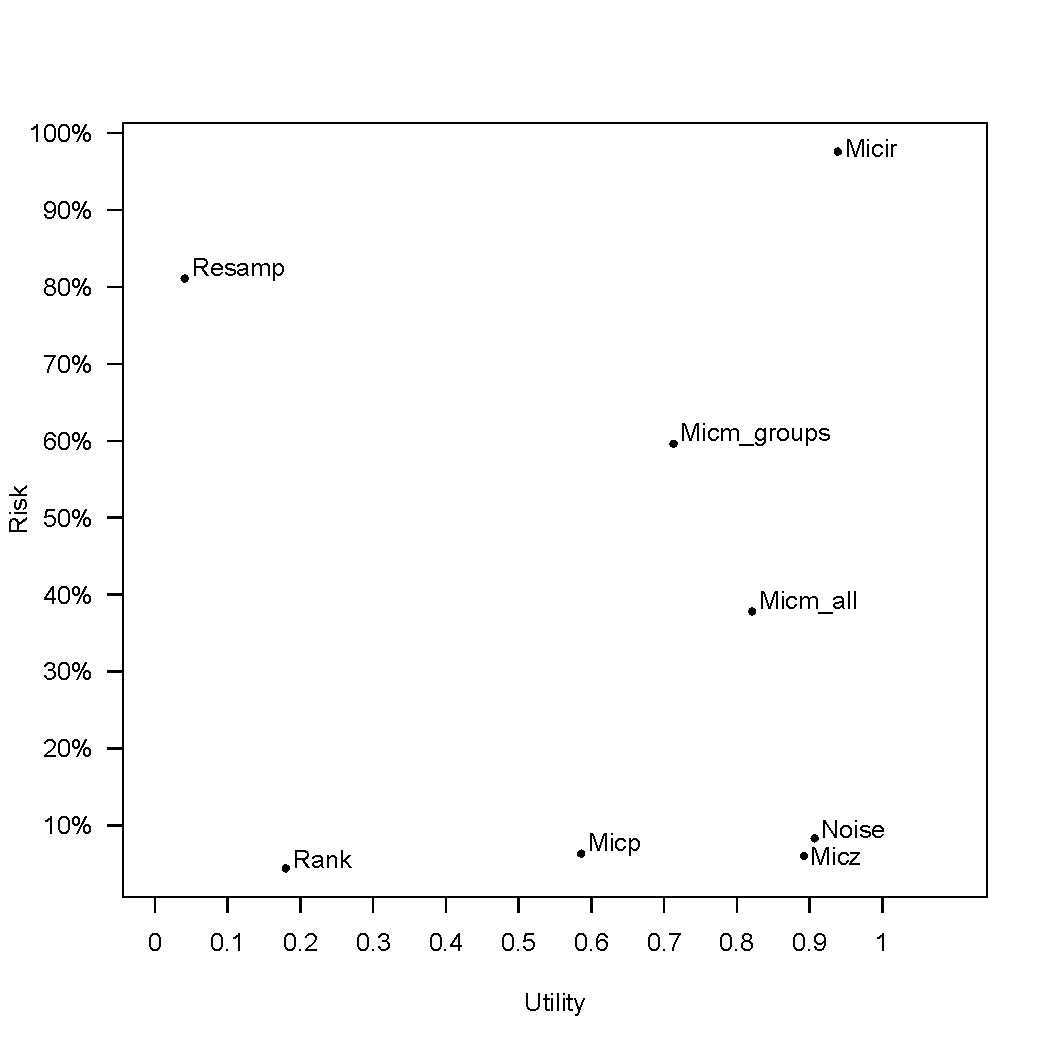
\includegraphics[width=4in]{R_U_plot.pdf}
\end{center}
\caption{Risk-Utility plot}
\label{fig.ruplot}
\end{figure}



%\section{Scope of this chapter}\label{sec:scope}

%We reference previous chapters' coverage of \gls{SDL} and other methods that restrict access to the full confidential 
%84
% data, describe various metrics that might be used to assess the utility of such methods.



\section{Evaluation metrics}\label{sec:overview_metrics}


\begin{figure}
    \centering
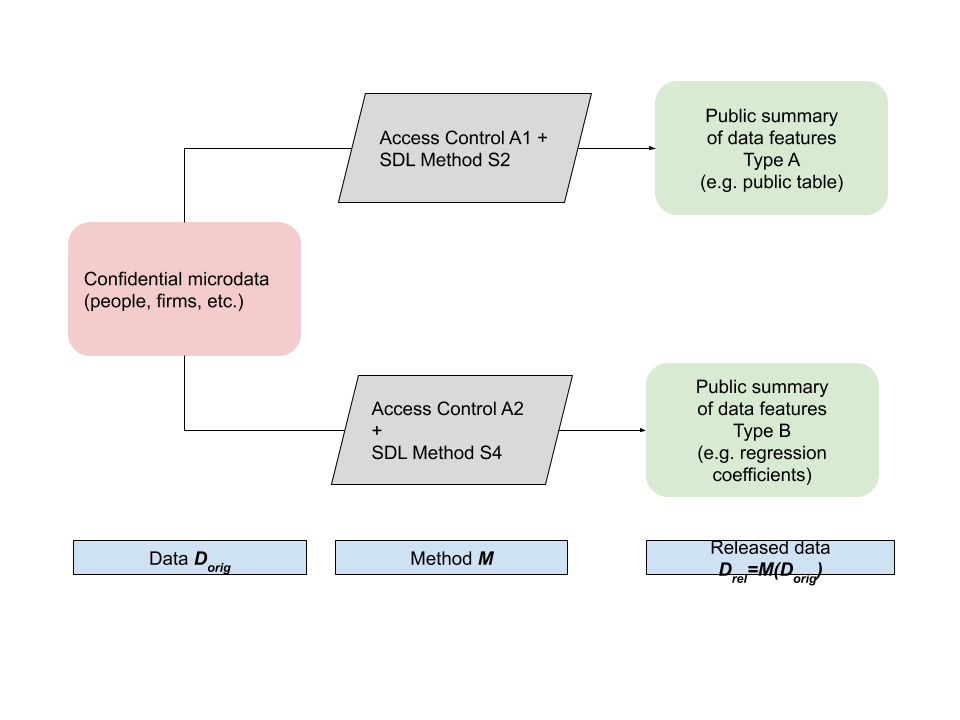
\includegraphics[width=0.8\textwidth]{SDL+Access control.png}
    \caption{Evaluation Framework}
    \label{fig:framework}
\end{figure}

\subsection{Non-Data Utility Metrics}\label{sec:other_metrics}
In assessing the utility of a particular method, a data custodian may also want to balance additional measures in conjunction with risk and utility. Examples include

\begin{itemize}
    \item Ease of access
    \item Timeliness of outputs
    \item Eligibility breadth
    \item Cost
\end{itemize}

\paragraph{Ease of access}

Ease of access seems to be correlated with user satisfaction for a given level of utility. Public-use data (in the public domain) provide great ease of access: in general, they can simply be downloaded. As restrictions are imposed, ease of access declines. Even agreeing to a very liberal license (such as the \href{https://creativecommons.org/licenses/by/4.0/}{Creative Commons Attribution 4.0 International (CC BY 4.0)} license, which requires attribution of the source by users) via a click-through agreement may prevent machine-readability of the download mechanism. More involved user agreements, requiring user input, or even institutional agreement, further reduce the ease (and speed, see below) of user access. The typical virtual or physical enclave may have weeks if not months of controls associated with access. 

Another important aspect is the ease with which the typical user community can leverage the provided data. Even public-use data may need to be accessible, via thorough data documentation and potentially adherence to a \textbf{community data schema} (refs here). Remote computing environments - enclaves, tabulation engines, and remote-submission systems - impose additional constraints. A remote submission system may be unfamiliar to many users. Remote desktop systems may provide limited software support, and may not be compatible with some users' expectations. For instance, as of 2020, few social science students are trained in \SAS{}, and yet several remote processing systems rely on \SAS{}. Conversely, many social science students are not yet trained in Python, and some newer systems in turn rely on those. 

\paragraph{Timeliness of outputs}

When access is granted, output controls may still vary, depending on the chosen method. For instance, a licensing scheme that delegates output control to the researcher may allow for very rapid release cycles, whereas a person-mediated disclosure avoidance system with limited capacity will delay output releases by days or months in the worst case. This may make a system with lower granularity but higher release speed more attractive to some users. 


\paragraph{Eligibility}

In general, eligibility of access may be limited. Many current restricted-access systems are limited to academic researchers, or at a minimum impose that outputs be made public-use. Whereas in the United States, much data is in the public-domain, imposing no restrictions on usage, in other countries, the lowest level is often a university-centric liberal licensing system (German campus files, until recently the Canadian Data Liberation Initiative). Such systems exclude community researchers, journalists, or commercial use, unless such users collaborate with eligible users. Conversely, even among academics, various levels of access restrictions may exist. In some instances, \footnote{VERIFY - true for HRS - which is not a federal survey.} the principal investigator must be a tenure-track faculty member, potentially excluding non-tenure-track researchers and lecturers. In other countries, students may be able to get restricted-access data with greater ease than tenure-track faculty (example: Canadian RDC system).

\paragraph{Cost}

Some systems will cost more than others, whether that is through computing infrastructure costs, compliance costs (contracts and such), or in costs imposed on users (e.g., travel costs to fixed locations for access such as RDCs). Depending on whether cost sharing (or billing) can occur, this may inhibit use. Maintenance of user-side infrastructure (such as support for RDCs or infrastructure fees for secure infrastructure) may limit accessibility only to institutions with greater financial capacity. 



\subsection{Data Utility metrics} \label{du_metrics}
In this section we present some examples of Data Utility metrics \DU\ that can be used by the data protector to assess the quality of the masked data, which can help to choose an appropriate approach for disclosure limitation.

In the broadest sense, the utility of a particular data release is the
benefit to society of the released information. Benefits this general
are nearly impossible to quantify and measure, because they depend on
more than simply the released data. A narrower, more feasible approach
is to characterize the quality of what can be learned from the masked
data relative to what can be learned from the original data. Such
comparisons can be tailored to specific analyses or can be broadened
to global differences in distributions. Examples of both approaches are presented in the corresponding sections below.

\subsection{Generic metrics of Data Utility}

Generic metrics capture global differences between the distributions of the original and masked data. 
One class of examples of generic measures are functions of the differences between point estimates of the first and second moments (and possibly other summaries) based on the original and masked data. Another is statistical distances between the distributions of the original and masked data \cite{dfks02, gks06}, for example Kullback-Leibler divergence.  When the data are approximately multivariate normal, the \KL\ captures the differences in the distributions of the entire data,
which in turn account for differences in inferences. 
However, the \KL\ measure is not easily
interpreted when the data, or some transformed version of the
data, are not reasonably well-described by a multivariate normal
distribution, that is why it's  usage as  global metric of data utility
would be limited.



\subsubsection{Propensity score utility metric}
% AO 03/31: start editing from here next time

An example of global utility metric that can be computed for the variables of different types is a propensity score based measure(\cite{propen}).

For any binary variable $T$, the propensity
score is defined as the probability that $T=1$ given covariate values $\bx$. \cite{rr83} show
that $T$ and $\bx$ are conditionally independent given the propensity
score. Thus, when two large groups have the same distributions of
propensity scores, the groups should have similar distributions of $\bx$.

This theory suggests an approach for measuring data utility.
First, we merge (by ``stacking'') the original and masked data sets, adding a variable $T$ that equals one for all records from the masked data set and equals zero for all records from the original data set. If
variables have been dropped as part of the masking, they are also
dropped in computation of propensity scores.  Second, for each record
in the original and masked data, we compute the probability of being
in the \textit{masked} data set---the propensity
score. Third, we compare the distributions of the propensity scores in
the original and masked data.  When those distributions are similar,
the distributions of the original and masked data are similar, and so
data utility should be relatively high.

Propensity scores can be estimated via a logistic regression of the
``masked/original'' variable $T$ on functions of all variables $\bx$
in the data set.  

The similarity of the propensity scores for the masked and original
observations can be assessed in numerous ways, for example comparisons
of their percentiles in each group.  A simple summary was proposed in \cite{propen}:
\begin{equation}
U_p =  \frac{1}{N} \sum_{i=1}^{N}\left[\hat{p}_i-c\right]^2,
\end{equation}
where $N$ is the total number of records in the merged data set,
$\hat{p}_i$ is the estimated propensity score for unit $i$, and $c$
equals the proportion of units with masked data in the merged data
set. In many cases, the original and masked data sets would have the
same size $N_0$, in which case, $N = 2N_0$ and $c = 1/2$. When the
original and masked data have the same distribution, the propensity
scores for all units should approximately equal $c$, so that $U_p$ is
near zero. At the other extreme, if $\hat{p}_i$ is nearly one for
units $i$ from the masked data and nearly 0 for units from the
original data, then the two data sets are completely distinguishable
and $U_p \sim 1/4$.


This measure is sensitive to the specification of the logistic
regression used to estimate the propensity scores.  For example, using
an intercept only in the regression results in $\hat{p}_i = c$ for all
$i$, regardless of the values in the masked data.  The advice from the
literature on propensity score estimation is
useful in the data utility context as well: include all variables,
with interactions and polynomial terms, considered important to make
similar in the original and masked data.

Note, that propensity score metric is not tied to the nature of the
masking.  This allows us to compute utility values on the same scale
for any masking strategy, which facilitates comparisons of the data
quality achieved by competing strategies applied on the same data
set.

Also note, that generic metrics of data utility may be blunt in that they do not necessarily distinguish among variables. For example, an \SDL\ procedure that produces very different distributions for a subset of substantively important predictors, but matches well on the subset of substantively unimportant predictors, could be rated as higher utility than a procedure that produces the opposite effects.  Similarly, minimizing the value of the generic utility metric may not lead to optimal \DBREL\ for certain conditional distributions.  

\subsection{Analysis specific metrics}
In this section we describe several analysis-specific or so called ``narrow'' measures of data utility. There are many possible ways of defining such type of metrics,  they 
are linked to the types of analyses the user would like to do on the original data.
 Obviously, we cannot cover all of them, so below we present some examples 
 that can help to illustrate the idea of such metrics.



\subsection{Confidence Interval Overlap Utility Measures}\label{subsec.ci}

Data users and analysts  are frequently interested in fitting regression models. 
This process produces not only point estimates of the coefficients, but
confidence intervals as well. Thus, it is desirable for utility measures 
to indicate when the inferences, and
not just the point estimates, from regressions using the released
data are close to the corresponding ones using the original data.

Confidence intervals are main mechanism of inference in regression
models. Therefore, one measure of utility is the degree of overlap
between confidence intervals obtained from the same regressions
fit using the \DBREL\ and \DBORIG. The greater the overlap, the
higher the utility.

\subsubsection{Interval Overlap Metric}
Consider a fixed regression on the data, with specified response
and predictors. Let $(L_{\mathrm{rel},k}, U_{\mathrm{rel},k})$ be
the lower and upper limits of the 95\% confidence interval for the
regression coefficient $\beta_{k}$ obtained from \DBREL, and let
$(L_{\mathrm{orig},k}, U_{\mathrm{orig},k})$ be the corresponding
interval obtained from \DBORIG. Let $f_{\mathrm{rel},k}$ and
$f_{\mathrm{orig},k}$ be the estimated posterior distributions of
$\beta_k$ computed under \DBREL\ and \DBORIG, respectively.  For
example, in linear regression, $f_{\mathrm{orig},k}$ is the usual
$t$-distribution on $n-p$ degrees of freedom with mean
$\hat{\beta}_{\mathrm{orig},k}$ and variance the $k$th diagonal
element in
$\hat{\sigma}^2_{\mathrm{orig}}\left(X^{'}_{\mathrm{orig}}
X_{\mathrm{orig}}\right)^{-1}$, where
$\hat{\sigma}^2_{\mathrm{orig}}$ is the estimated residual
variance obtained from fitting the regression of
$Y_{\mathrm{orig}}$ on the associated $n \times p$ matrix of
predictors, $X_{\mathrm{orig}}$, which includes a vector of ones
for the intercept.

The probability overlap in the confidence intervals for
any $\beta_{k}$ \citep{kkors06} is defined to be equal to:
\begin{equation}
I_k = \frac{1}{2}
\left[\int_{L_{\mathrm{rel},k}}^{U_{\mathrm{rel},k}}
f_{\mathrm{orig},k}(t) dt +
\int_{L_{\mathrm{orig},k}}^{U_{\mathrm{orig},k}}
f_{\mathrm{rel},k}(t) dt \right]
\end{equation}
and the interval overlap measure, \IO, as
\begin{equation}
I = \sum_{i=1}^p I_k / p
\end{equation}
where $p$ is the dimension of the predictor variable matrix, including
the intercept.

By design, $0 \leq I_k \leq 0.95$ (as is the case for $I$), with
effectively no overlap corresponding to $I_k =0$ and perfect
overlap corresponding to $I_k = 0.95$.  Averaging the two
integrals in the definition of $I_k$ helps deal with cases where
$(L_{\mathrm{orig},k}, U_{\mathrm{orig},k}) \subseteq
(L_{\mathrm{rel},k}, U_{\mathrm{rel},k})$, or vice versa.  For an
illustrative example, consider the case where
$(L_{\mathrm{orig},k}, U_{\mathrm{orig},k}) = (8, 10)$, and for
two different proposed releases the $(L_{\mathrm{rel_1},k},
U_{\mathrm{rel_1},k})=(-12, 30)$ and $(L_{\mathrm{rel_2},k},
U_{\mathrm{rel_2},k})=(3, 15)$. From a utility perspective, the
second release is clearly preferable over the first release. The
\IO\ as defined favors the second release.  A criterion that just
equals $\int_{L_{\mathrm{rel},k}}^{U_{\mathrm{rel},k}}
f_{\mathrm{orig},k}(t) dt$ does not clearly distinguish the
releases, since this integral for both procedures is essentially
one. Similar examples can be constructed to show the inadequacy of
using $\int_{L_{\mathrm{orig},k}}^{U_{\mathrm{orig},k}}
f_{\mathrm{rel},k}(t) dt$ alone.

The \IO\ does not distinguish among intervals that have $I_k$
essentially equal to zero, some of which may be ``less worse''
than others. To adjust for this, the measure can be modified by
adding some distance-based penalty when $I$ is essentially zero,
or perhaps even when $I_k$ is essentially zero for some $k$, where
distance is defined as some function of the
$|\hat{\beta}_{\mathrm{rel},k} - \hat{\beta}_{\mathrm{orig},k}|$
or of $\min\left\{|L_{\mathrm{rel},k} - U_{\mathrm{orig},k}|,
|L_{\mathrm{orig},k} - U_{\mathrm{rel},k}|\right\}$.

An alternative measure is the overlap in the interval lengths. Let
$(L_{\mathrm{over},k}, U_{\mathrm{over},k})$ be the overlap in
these intervals, defined as $\left\{b: b \geq L_{\mathrm{orig},k},
b \geq L_{\mathrm{rel},k},  b \leq U_{\mathrm{orig},k},  b \leq
U_{\mathrm{rel},k}\right\}$. Then, the average relative overlap in
the confidence intervals for any $\beta_{k}$ equals:
\begin{equation}
J_k = \frac{1}{2} \left[\frac{U_{\mathrm{over},k} -
L_{\mathrm{over},k}}{U_{\mathrm{orig},k} - L_{\mathrm{orig},k}} +
\frac{U_{\mathrm{over},k} -
L_{\mathrm{over},k}}{U_{\mathrm{rel},k} -
L_{\mathrm{rel},k}}\right].
\end{equation}
The interval overlap measure then could be defined as $J = (1/p)
\sum_{i=1}^p J_k$.

\subsubsection{Ellipsoid Overlap Metric}\label{subsec.overlap}
The \IO\ measure considers each interval separately, effectively using all
the conditional distributions of the coefficients rather than
their joint distribution. Some analysts may be interested in
simultaneous intervals, which are defined by multidimensional
ellipsoids.  So, ellipsoid overlap measure \EO\ is constructed 
based on  posterior probabilities of regions defined by ellipsoids, that is, 
Bayesian perspective is used.  Generically, let $\hat{\beta}$ be the
maximum likelihood estimate of $\beta$, the $p \times 1$ vector of
true coefficients in the regression of $Y$ on $X$, and let
$\hat{\sigma}^2$ be the estimated residual variance for that
regression. Under the standard linear regression assumptions and
assuming standard non-informative prior distributions for $\beta$
and $\sigma^2$, the $(1-\alpha)100\%$ joint highest posterior
density ellipsoid for $\beta$ is defined by all the values of
$\beta$ such that
\begin{displaymath}\label{eq_1}
\frac{(\beta
-\hat{\beta})^T(X^{T}X)(\beta-\hat{\beta})}{p\hat{\sigma}^2} \leq
F(\alpha;p, n-p)
\end{displaymath}
where $F(\alpha;p, n-p)$ is the critical value from the $F$
distribution with $p$ and $n-p$ degrees of freedom.  The ellipsoid
from the \DBORIG, which we call $E_{\mathrm{orig}}$, is obtained
by setting $\hat{\beta} = \hat{\beta}_{\mathrm{orig}}$,
$\hat{\sigma}^2 = \hat{\sigma}^2_{\mathrm{orig}}$, and $X =
X_{\mathrm{orig}}$. The ellipsoid from the \DBREL, which we call
$E_{\mathrm{rel}}$, is obtained by setting $\hat{\beta} =
\hat{\beta}_{\mathrm{rel}}$, $\hat{\sigma}^2 =
\hat{\sigma}^2_{\mathrm{rel}}$, and $X = X_{\mathrm{rel}}$.

The utility measure \EO\ is the average of two posterior
probabilities: 1) the probability of $E_{\mathrm{orig}}$ computed
using the posterior distribution of $\beta$ based on \DBREL, and
2) the probability of $E_{\mathrm{rel}}$ computed using the
posterior distribution of $\beta$ based on \DBORIG. To determine
these probabilities,  Monte Carlo simulations can be used. For the first
probability, we draw values of $\beta$ from its posterior
conditional on \DBREL\ which is a $p$-variate t-distribution with
mean $\hat{\beta}_{\mathrm{rel}}$ and covariance matrix
$\hat{\Sigma}_{\mathrm{rel}} =
\hat{\sigma}^2_{\mathrm{rel}}(X_{\mathrm{rel}}^{t}X_{\mathrm{rel}})^{-1}$
with $n-p$ degrees of freedom. We then calculate the percentage of
these drawn $\beta$ that lie within $E_{\mathrm{orig}}$.  A
similar process is used to obtain the second probability by
drawing from the posterior of $\beta$ given \DBORIG\ and finding
the percentage of these that lie inside $E_{\mathrm{rel}}$. As
with \IO, the \EO\ can be extended to any parameters whose
distribution is well-approximated by a multivariate normal
distribution.

\subsection{Privacy metrics}\label{sec:privacy_metrics}
Placeholder

% Here: start removing from here or drastically reducing, we may just say that 
% such and such methods have generally such and such utility or compare in such a way with other methods,
% say noise is better than mixroaggregation and microaggregation is better than swapping - or simething like that.

\section{On Utility Properties of some families of \SDL\ methods}
\label{subsec.simulateddata}

There is a wide plethora of SDL methods and they differ significantly in terms of utility  and risk. Moreover, each method can be applied with a different degree of intensity, that is, data protector can chose  different values of parameters for these methods which leads to a significant variability in terms of utility for the same type of SDL method. 
For example, for Noise addition, smaller or larger variance of Noise can be chosen, which will affect the utility and risk of the masked data. For Swapping, the percentage of swapped records can be different; for Rankswappping  the  maximal allowed difference in the ranks of the swapped records  may vary (which is a parameter of Rankswapping). For Microaggregation, a minimal number of records per group, which is a parameter of microaggregation, can significantly affect the utility of the data, as microaggregation has a shrinkage effect on the data. Thus the number of method-parameter combinations is virtually infinite, each one with it's own utility and risk. Hence, it is impossible to provide a comprehensive utility comparisons of method-comparisons combinations. Thus, we will present generic utility characterizations for a small selection of well known families of SDL methods. 

\subsection{Microaggregation}
One of the largest families of SDL methods (in terms of different  implementations) is a  Microaggregation family. It can   be divided into Multivariate Microaggregation   and  Univariate Microaggregation. The later group includes Microaggregation with individual ranking which consists of microaggregating each variable individually and independently from other variables and Microaggregation using projections. The later one is usually accomplished by ranking  multivariate data by projecting them onto a single axis, using either the sum of $z$-scores or the first principal component, and then aggregating data into groups of size $k$, except possibly for one group of larger size (from $k+1$ to $2k -1$).
Of all these methods, Microaggregation with individual ranking is typically the least perturbative method \citep{kkors06}. Typically, masked values obtained using this method are close to the corresponding original ones, and thus analyses performed on the masked data often lead to a very similar results to those obtained on the original data. For example, \EO\ utility metric is often high (close to $1$)  for this method \citep{kkors06}. On the other hand, the risk of re-identification using record linkage approach is high for this method as well. 
In contrast to Microaggregation using Individual Ranking, projection-based Microaggregation methods and Multivariate Microaggregation may introduce significant perturbation to the data with utility ranging from average to low according to \IO\ and \EO\ . But the re-identification risk (estimated based on record-linkage experiments) is low as well \citep{}. 

One of the desirable features of Microaggregation methods is that they  inherently satisfy requirements of $k$-anonymity (if this criterion for Risk  is adopted by the data protector of course). Also microaggregation methods preserve means of the original data, they preserve positivity/non-negativity  constraints in the data (if the original values are positive, so are the masked values)  which in some instances of data release  is a desirable feature. Microaggregation methods, on the other hand have a shrinking effect on the original data by reducing  the variance of the original data.

\subsection{Coarsening}
Coarsening and rounding. To be filled in.
 
\subsection{Noise addition/multiplication} 

Another large family of methods is Noise infusion, which can be implemented as additive or multiplicative noise for numerical variables.
Some implementations of noise infusion, for example additive multivariate normal noise, followed by the data transformation \cite{} or multiplicative log-normal noise \cite{} also followed by the data transformation, preserves the mean vector and covariance matrix of the original data on average. These statistics are important for a range of analyses, for example, for linear regression. In general, noise infusion does not preserve positivity constraints for the variables and inter-attribute relationships such as linear inequalities. For example, Age, many
economic variables(gross income, taxes) and many demographic variables (number of employees, number of students in the sixth grade) obey positivity constraints. Examples of inequality constraints are ``Federal taxes $<$ gross income’’, ``number of salaried employees < number of employees'' and ``year of birth < year of death''.

% AO start here next time!


For example, , that is, if original variables are non-negative then masked variables are also non- negative. Multiplicative noise on the other hand can preserve positivity constraints.
 % Here: About metric-related performance of noise.
 
Standard implementations of additive and multiplicative noise does not satisfies the requirements of $k$-anonymity.
Noise generated from Normal distribution with specially calibrated variance, as well as noise generated from Laplace distribution with special parameters  satisfies requirements of  differential privacy.
Record linkage experiments showed that additive noise has low re-identification risk.

\subsection{Swapping}
{\bf To be filled later}...


\subsection{Synthetic methods}
{\bf To be filled later}...

 
\section{{Restricted Data Access Models and the Effect They Have on Data Quality and Usability}}


\subsection{ACCESS TIER: PROTECTED}
\begin{itemize}
\item{Restricted-use data behind firewall with output controlled for disclosures};
\item{Automated output from SDL software with use restrictions} E.g. web-based query system.
\item{Licensing program} User controlled infrastructure.
\end{itemize}

Access to this data is not automatic but requires one or more additional steps such as, but not limited to, a data use agreement, license, system or website account, and automated SDL tools with built-in limitations on allowable output. The number of additional requirements for access is intended to be more than the public access, but less burdensome than the restricted tier. The lowered burden should improve access, timeliness, and other aspects of data quality in a meaningful way to the data customer.

\subsubsection{Web-Based Query Systems} 
Query systems allow users to design queries to generate customized tabulations (WP 22). Also have predefined queries.
Data stored in query systems can be protected and restricted.






\paragraph{Nonstatistical Metrics}
\begin{itemize}
    \item  Expensive to implement and maintain (Haggard, 2006, 189)
   \item Functionality is limited to what the developer allows to be run in the query system
   \item No direct access to the microdata (may vary by agency)
   \item Decrease utility
   \item May not prevent disclosures (table splicing; can do this in CDC Wonder) 
   \item Functionality is limited to what the developer allows to be run in the query system
   \item Developer can build in SDL (see Gomatam, 2005, 167)
\end{itemize}

\paragraph{Statistical Metrics}
\begin{itemize}
    \item    Built in disclosure technique can reduce utility and quality (Gomatam, 2005, 167-168)
     \begin{itemize}
         \item  Top coding, \gls{swapping}, \gls{output_noise_injection} (adding noise) (WP 22)
        \item Prohibit key identifiers (age, race, sex) as outcome variables but permit as predictors (Gomatam, 2005, 167)
       \item Disallow certain transformations (Gomatam 2005, 173)
       \end{itemize}
   \item Run queries on data more detailed than PUFs (varies by agency—could be restricted data or perturbed data from public use files) 
   \begin{itemize}
     \item Increases utility, improves data quality
     \item Permits a wider range of analyses than does releasing only data summaries and it provides results based on actual rather than simulated microdata (Gomatam, 2005, 164)
   \end{itemize}
\end{itemize}











Examples of online query systems: 
\begin{itemize}
\item 	NASS (Karr)
\item 	Australian Bureau of Statistics, TableBuilder (Chipperfield, 2019)
\item 	CDC’s Wonder
\item 	BLS ??
\item The \href{https://microdata.no}{microdata.no} system provides a facility to analyze Norwegian register data. The system allows for descriptive statistics as well as a small set of regression methods and  analysis of variance. Automated anonymization processes have been implemented, and microdata cannot be viewed. Researchers must be affiliated with (Norwegian) institutions having an agreement with Statistics Norway. A custom programming interface is used, based on Python augmented with four (commonly used) Python modules, but limited to certain functionality. 
\end{itemize}




\subsection{ACCESS TIER: RESTRICTED ACCESS}
\begin{itemize}
\item{Licensing program} (user controlled infrastructure)
\item{Virtual Data Enclave}
\item{Physical Data Enclave}
\end{itemize}

Virtual and Physical Data Enclaves







This is the default tier for containing data collected under a pledge of confidentiality. Critical to its modernization is to include more access options using newer technology such as commercial cloud computing and remote access/virtual enclave. This should also include viable options not constrained by the current system of Federal Statistical Research Data Centers (FSRDCs).

\subsubsection{Virtual and Physical Data Enclaves }
There are two types of \glspl{data-enclave}: 1) \glspl{physical-data-enclave}; and 2) \glspl{virtual-data-enclave}. Both types of enclaves allow researchers to access restricted use data under highly restricted conditions which reduces disclosure risks. Some data enclaves allow researcher to access the full data sets while others require researchers to prepare data dictionaries and limit access to only the variables the researchers need to complete their analysis. 

The primary difference between the two types of data enclaves is the process by which the data are accessed. In physical data enclaves researchers must physically sit in a controlled environment at the data owner’s office or site where the data are stored. Virtual data enclaves allow researchers to access the restricted use data remotely over secure electronic lines via their personal computers while they sit in their own offices or homes. The output generated is returned to the researchers.

Both types of data enclaves increase the usability of the data. Researchers are permitted to access data not publicly available under controlled conditions. For example, [list types of data that cannot be publicly accessed: genetics data, geocoded data, detailed geography, exact dates, detailed race, income]. 

\begin{comment}
Conversely, both types of data enclaves can also decrease the utility of the data. The process for requesting access to restricted use data can be arduous and thus reduce the number of researchers who can access the data. Researchers must submit research proposals containing detailed information about the research project, the hypotheses to be tested, the data set and variables to be used in the analysis,
the empirical methods to be used, and the specific data outputs that will result from the project thus limiting exploratory analyses. Research proposals are reviewed and approved by a review committee which can take several weeks or months to complete. Additionally, users must agree to terms and conditions governing the access and use of the confidential data as well as sign nondisclosure affidavits. Some researchers are required to complete background investigations, Special Sworn Status, be citizens of the U.S.,  …etc.  Furthermore, there are costs associated with accessing restricted use data via data enclaves [include examples]. Costs reduce the utility of the data because some researchers may not have funding to complete research. Most students completing graduate or doctoral level research, living on fixed incomes, may not be able to afford to access data in enclaves. 

Both types of data enclaves allow researchers to improve the accuracy and precision of their estimates. Data available in enclaves are not subject to the statistical disclosure limitation methods that public use files are subject to prior to release. For example, detailed race/ethnicity and geography measures are typically not available on public use files due to disclosure concerns. These types of measures are available to researchers in data enclaves thus increasing the accuracy and prevision of estimates.  [Might include examples of research completed in RDCs that could not be completed using PUFs].

Data quality can also be decreased when accessing restricted use data in data enclaves. Extreme values or values representing an individual are generally removed from analysis (e.g. minima, maxima, medians). These values might be useful to researchers doing sensitivity analysis. {need to expand this section}
\end{comment}

\paragraph{Examples of physical enclaves}
\begin{itemize}
    \item BLS and NCHS each have a ``research data center'' at their headquarters, which are physical enclaves (?)
\end{itemize}

\paragraph{Examples of virtual enclaves}
\begin{itemize}
    \item The \href{https://www.norc.org/Research/Capabilities/Pages/data-enclave.aspx}{NORC Data Enclave} is used by the two \href{https://www.norc.org/Research/Projects/Pages/usda-ers-data-enclave.aspx}{USDA statistical agencies}
    \item The Inter-university Consortium for Political and Social Research (ICPSR) Virtual Data Enclave is used by the \href{https://www.icpsr.umich.edu/icpsrweb/content/NACJD/index.html}{Bureau of Justice Statistics' National Archive of Criminal Justice Data}. 
\end{itemize}

\paragraph{Examples of hybrid enclaves}
\begin{itemize}
    \item the FSRDC system is accessed from secure rooms, which in turn provide access to a secure network, with all data stored in a central location. It is thus a hybrid of a physical enclave housing a virtual enclave. About a dozen statistical agencies provide access to some of their data through this system. Output control varies by agency.
    \item the French system \href{https://casd.eu}{Centre d'acc\`es s\'ecuris\'e de donn\'ees (CASD)} is a virtual enclave, with access devices typically restricted to dedicated physical devices located in university offices. Much of French administrative data can be accessed through this system. Output control varies by agency.
    \item the \href{https://fdz.iab.de/}{German Research Data Centre (FDZ)} of the German Federal Employment Agency (BA) at the Institute for Employment Research (IAB) uses multiple access modes, one of which has dedicated thin clients located in designated access-controlled offices (typically at universities), connecting to an agency-controlled virtual desktop infrastructure. Output control is manual.
\end{itemize}




\paragraph{Nonstatistical Metrics}

\begin{itemize}
    \item Accessibility (level of difficulty)
    \begin{itemize}
         \item Physical RDC: Must physically sit in RDC to access RU data.
        \item Virtual RDC: Access RU data remotely over secure electronic lines via personal computers while sitting in office or home.
    \end{itemize}
    \item Increase utility of data (access to data not otherwise accessible) 
    \begin{itemize}
         \item Genetics data, geocoded data, detailed geography, exact dates, detailed race, income
    \end{itemize}
    \item Decrease utility of data
    \begin{itemize}
        \item        Process to obtain access is arduous
        \begin{itemize}
             \item Prepare research proposals
            \item Review committees (can take several weeks, months to complete)
            \item Agree to terms and conditions of use: 
           Sign affidavits, 
           Complete background investigations, Special Sworn Status, be citizens of the U.S.,  
           Etc.
        \end{itemize}
    \end{itemize}
    \item Costs (include examples)
    \begin{itemize}
        \item        Some researchers may not have funding to complete research. Most students completing graduate or doctoral level research, living on fixed incomes, may not be able to afford to access data in enclaves.
    \end{itemize}

\end{itemize}



\paragraph{Statistical Metrics}
\begin{itemize}
    \item      Improve the accuracy and precision of estimates
    \begin{itemize}
          \item Data available in enclaves are not subject to the statistical disclosure limitation methods that public use files are subject to prior to release. For example, detailed race/ethnicity and geography measures are typically not available on public use files due to disclosure concerns. These types of measures are available to researchers in data enclaves thus increasing the accuracy and prevision of estimates. 
         \item Might include examples of research completed in RDCs that could not be completed using PUFs (example: top-coding of income and inequality measures, in ACS)
    \end{itemize}
    \item Decrease data quality (maybe include?)
    \begin{itemize}
         \item    Extreme values or values representing an individual are generally removed from analysis (e.g. minima, maxima, medians). These values might be useful to researchers doing sensitivity analysis (need to expand this section). This varies by RDC. 
    \end{itemize}
    \item Include a discussion on how/if RDCs subject restricted use data to statistical disclosure methods
    \begin{itemize}
            \item NCHS RDC does not apply SDL methods to data. They do apply complementary cell suppression
            \item BLS RDC does top code some data (check with Ellen on this)
            \item Census applies \gls{coarsening} to some data (geography), censors name and address information for most data unless expressly allowed
    \end{itemize}
\end{itemize}



\subsubsection{Licensing Program (user controlled infrastructure)}

Licensing agreements permit a researcher to use restricted data offsite, but under highly restricted
conditions, as spelled out in a legally binding agreement [text from Restricted Access Procedures]. Arrangements that place restrictions on who has access, at what locations, and for what purposes access is allowed normally require written agreements between agency and users. These agreements usually subject the user to fines, being denied access in the future and/or other penalties for improper disclosure of individual information and other violations of the agreed conditions of use. Users may be subject to external audits conducted by the agency to assure terms of the agreement are being followed. Users in violation may be required to pay fines or be subject to other legal penalties [text from WP 22].







\paragraph{Examples}
\begin{itemize}
    \item NCES provides access to certain data sets through a licensing scheme. Additional information on this method is provided here: \url{https://nces.ed.gov/FCSM/pdf/CDAC\_RAP.pdf}
    \item Various agency-sponsored surveys, such as the National Longitudinal Surveys of Youth (NLSY) may provide access to certain elements of otherwise public-use microdata via a licensing scheme. For instance, the NLSY79 Geocode Data is subject to a \href{https://www.bls.gov/nls/questions-and-answers.htm#anch25}{variant of a licensing program}. Note that yet other data may only be available through more restricted access methods, such as enclave data.
\end{itemize}



\paragraph{Nonstatistical Metrics}

\begin{itemize}
    \item Arduous process (text from Restricted Access Procedures)
    \item  Demonstrate a need for sensitive data
    \item  Need to provide authorization for all users at the requesting institution 
    \item Signatures by senior level official and key staff.
    \item Submit data security plan
    \item Data provider may want to review statistical output before publication’
    \item  IRB review, approval might be needed
    \end{itemize}
Note: should include text here regarding Designated Agent Agreements for CIPSEA protected data.

\paragraph{Statistical Metrics}

     See statistical metrics for virtual and physical RDCs
     Others?



\begin{comment}
Licensing agreements require:
\begin{itemize}
\item a demonstrated need for sensitive data;
\item authorization for all users at the requesting institution;
\item signature by a senior level official and key staff;
\item a data security plan;
\item agreement by researchers not to identify individual research subjects or to link data received with other microdata files; and
\item typically review of all statistical output before publication, though licensing agreement delegate this to the requesting institution (researchers)
[text from Restricted Access Procedures].
\item 
The license may be for a specified period of time and data files must be returned or destroyed. 
\item Some licensors require fees and/or approval by an institutional review board. 
\end{itemize}


\paragraph{Pros for Licensing Program}
\begin{itemize}
    \item Provides for flexibility in terms of analysis methods and user computing infrastructure
    \item Because no computer infrastructure needs to be set up to support access, relatively low-cost method
\end{itemize}

\paragraph{Cons for Licensing Program}

\begin{itemize}
    \item Loss of control over data security, mitigated by inspections
    \item Potential loss of control over output control
\end{itemize}

\end{comment}


 

\subsubsection{Future Placeholder for Highly Restricted Access Tier}
(leave blank)



\section{Public Use Microdata (Ellen's stuff)}

**Note - Ellen will edit and add to this Thursday and add citations, but I wanted to add something for now.

Many statistical agencies provide microdata files directly to the public, available online without requiring users to register or provide information about what they will do with it. 

One advantage of making public use files available is that the data can reach a much wider audience and be used much more broadly. They are generally made free for anyone who would like access, which makes them particularly appealing for students and researchers alike.

Depending on the data, they can also be extremely easy for people to use and understand. While some may require extensive codebooks and statistical knowledge to manipulate, some government agencies are moving toward online query systems that allow anyone to determine information with little effort. For example, Baltimore city has a public database of all 911 calls that can be downloaded if the user would like to. However, they also have a query system on their website that allows users to look at combinations of variables, such as locations, date and times, and types of emergencies. With a few mouse clicks, any user can create a visualization of the data that can include multiple variables. 

Providing more people easier access to microdata can allow for more queries to be run, more data to be combined, and more research to be conducted that can change public policy. Most government agencies conduct marketing research and implement marketing techniques with the goal of having more people use their data, whether tabular or microdata. By allowing access to microdata, however, there is more information that can be gathered from the data, it can be used in additional ways, and has the potential to influence more research, more policies, and more people.

In addition, wide access to public use data can often allow for those datasets to be combined with other confidential datasets that likely wouldn’t be possible if the data were only available in a restricted use setting. Most restricted use access options, such as FSRDCs or virtual data enclaves, prevent users from removing the data in any means from their location. Public use files can usually be uploaded into these settings, but because it is not possible to pull the restricted use files from their location, it is often impossible to combine two restricted use files and draw conclusions from the resulting datasets. Public use files allow data users to combine the data with confidential datasets, which can result in conclusions that would not be possible to draw without public access to the data. 

Of course, the practice of making access to data easier, especially unperturbed microdata, increases the risk of it being used for malfeasance. Even data that are believed to be anonymized can often be used to determine information about specific respondents. Examples of misused public data are numerous, from determining preferences of Netflix users  to identifying the governor of Massachusetts in medical records by pairing it with public voter identification information . The Panel of Data Access for Research Purposes proposed two recommendations to limit de-identification attacks on government data. First, all users should be notified when accessing government data that it was collected with the legal requirement to be used for only statistical purposes and users should be required to acknowledge that they have read the disclaimer before the data can be viewed. Second, government institutions should impose ``meaningful’’ penalties for users who use the data for something other than statistical purposes, such as de-identification attempts. While that recommendation was made by the panel in 2005, many government agencies have not taken these steps and still allow access to their microdata without reading a disclaimer and have no real penalties in place for misuse of the data.

While the United States has decentralized statistical agencies which largely create their own rules on data access, other countries often have tiers of access that are standard for all data programs. Stats Canada, for example, has certain datasets that are available publicly and certain datasets that can only be accessed through data research centers or remote access that is granted for researchers. However, there are also certain datasets for which Stats Canada allows researchers to access tabular data by submitting statistical programs without seeing the underlying microdata, for which tabular data is returned. This intermediate data access level can allow the program to apply disclosure methods to the tabular data but allow researchers to use the microdata, which can add some protections for the respondents.

The United Kingdom Data Center has three levels of access, as well: open, safeguarded, and controlled data. Open data is believed to be completely free of identifying data and can be used by anyone without permission or registration. Safeguarded data is believed not to have identifying information, but there could be concerns about the possibility of identifying respondents by linking the information with other dataset. To gain access to these data, users need to register and agree to certain conditions, such as not using the data to identify individuals or disseminate any identifying information. Finally, controlled data is believed to contain information that could be disclosive and is protected through a number of means, such as requiring users to register and be approved, as well as complete training to access the data.

For both Stats Canada and the UK Data Center, each dataset is evaluated for risk and the microdata are assigned a level of protection. In some cases with risky data, the data are altered in some way, such as by removing variables, to decrease the risk. This can allow different versions of the same dataset to be available at different access levels, so researcher with training and appropriate credentials can gain access to the full data while other users who may not have the necessary credentials or may not need the full dataset can use the modified data. This gives the advantage of wide access to the data while protecting the most vulnerable elements of information from the respondents.

\subsection{Disclosure Protection in Public Use Files}

When datasets are release for public use, they generally have some modifications made to reduce risk to respondents. That does not mean that all risk is eliminated, but most government agencies at least attempt to limit the likelihood of re-identification. At the very least, this means removing respondent identifying information, such as names, addresses, and dates of birth from the data. In many cases, this is not removed from the file entirely, but changed into some sort of aggregate variable like county or state rather than address, or year of birth rather than exact date. While this helps to protect the respondents, it can also reduce the utility of the file. If state is the only information provided regarding the location of the respondent, it prevents studies of rural versus urban respondents.

In addition, many variables in public use microdata are rounded, top-coded, or organized into certain groups. Again, these methods may reduce some amount of utility, but can protect respondents. With the availability of information available that can be merged with public use data, exact information about variables such as dollar amounts, especially for outliers, can pose a risk. However, these methods can also skew; if wages are top-coded so all earnings above a certain level are written as something lower, the averages will no longer accurately reflect the overall population.

More surveys are beginning to use some form of data perturbation to create the microdata file that is released to the public. 
The American Community Survey (ACS) at the Census Bureau, which collects information from 2.3 million housing units per year, will move to creating synthetic data and release that as their public use microdata file, rather than the actual collected data. They have begun testing methods for creating the synthetic data, but so far, only some of the properties in the original data are reflected in the synthetic data. At geographic areas lower than the state, there are even fewer properties of the original data reflected in the synthetic microdata file.

Some surveys, such as the National Longitudinal Survey of Youth at the Bureau of Labor Statistics, release public use data files with most variables include, but lacking almost all geographic information. While that helps to provide protection for respondents to the surveys, it makes it impossible to make determinations about variations across locations.




\section{Data Access - from LARS}
\begin{center}
 DRAFT (C) Lars Vilhuber, Jim Shen - do not distribute    
\end{center}

\hypertarget{physically-protecting-sensitive-data}{%
\subsection{Physically Protecting Sensitive
Data}\label{physically-protecting-sensitive-data}}

The physical protection of sensitive data is one of the key parameters
that data custodians can and do influence. Within the Five Safes
Framework, ``safe settings'' are heavily influenced by how data are
physically protected. However, it is also the parameter that is most
dependent on current technology. While sending around floppy disks to
researchers who inserted them into desktop computers in a locked room,
isolated from computer networks, was common in the 1980s, it has been
superseded by technologies that provide similar or stronger security,
combined with greater ease of access.

Possibly because technological advances happen faster than legal or
cultural habits change, we have found that data custodians and policy
makers may not always be aware of the most current technological
possibilities when crafting the legal and contractual framework for data
access. This chapter sets out to describe the currently available
spectrum of physical protection methods. We use a framework that defines
five dimensions with which we can characterise a particular access
mechanism. We then describe several actual examples, both from the case
studies in this handbook as well as others that we are aware of.
Finally, we caution readers that by the time that this chapter is being
read, the range of possibilities may yet again have expanded (rarely
does it contract). Technological obsolescence is intrinsic to a chapter
relying so heavily on technology.

\hypertarget{five-dimensions-of-physical-security}{%
\subsubsection{Five Dimensions of Physical
Security}\label{five-dimensions-of-physical-security}}

In any data sharing setup, the fundamental setup always involves the
original holder of the data, and access by a new entity. In the context
of this Handbook, the original holder is the data custodian, and the new
accessor is the researcher. Technology determines how the physical
exchange and access may happen.

Here, we propose five dimensions of physical data security to serve as a
framework to evaluate the different defining features of various data
access mechanisms. These are:

\begin{itemize}
\tightlist
\item
  the physical \textbf{location of analysis computers and the data},
\item
  the \textbf{control over analysis computers} that researchers are
  allowed,
\item
  the \textbf{location and type of access computers},
\item
  the \textbf{level of security of access locations}, and
\item
  the \textbf{range of analysis methods available} to researchers.
\end{itemize}

When proposing and negotiating a potential use sharing agreement,
evaluating the physical security arrangements along these five
dimensions can help researchers and their data providers craft robust
mechanisms to protect data when transferring and using data for
research. Importantly, these physical access mechanisms in turn interact
with the other four safes. We highlight such interactions in the
examples provided.

For each dimension, classifications range from \textbf{1} to \textbf{3},
except for security, which has a range of \textbf{4}.

\hypertarget{location-of-analysis-computers-and-data}{%
\paragraph{Location of Analysis Computers and
Data}\label{location-of-analysis-computers-and-data}}

The researcher-accessible administrative data can be stored at one of
three types of locations. The data can remain with the data provider,
the data provider can transfer the data directly to the researcher, or
the data provider can transfer the data to a trusted third party. Each
possible data location comes with its own requirements, advantages,
disadvantages, and special considerations for the researcher and data
provider.

\begin{longtable}[]{@{}lll@{}}
\toprule
1 & 2 & 3\tabularnewline
\midrule
\endhead
Data provider & Third-party & Researcher\tabularnewline
\bottomrule
\end{longtable}

Key consideration for the choice of location is the level of trust that
the data provider has in the entity controlling the new location. The
enforcement of DUA or MOU is key. Transferring control to another entity
might be desirable when support for many researchers is a burden for the
regular business of the data provider. For instance, by transferring the
data to the researcher, a data provider may no longer be responsible for
the cost of providing computational infrastructure for data storage and
analysis. On the other hand, costs of enforcing access restrictions,
such as site visits, may be higher once physical custody of the data has
been transferred.

In certain cases, the transfer to a third party or the researcher
unlocks the possibility of combining data from multiple data providers.
For instance, government departments responsible for immigration and
taxes may not be legally allowed to share data, but they may each be
able to transfer the data to a national statistical office. Similarly,
multiple companies may not be willing (or legally allowed) to share data
with one another, but may be able to transfer the data to trusted third
party. In other situations, one branch within a government department,
responsible for enforcement, may transfer the data to another branch,
whose business it becomes to make the data accessible. The advantages of
this arrangement include having an organization that is more familiar
with and responsive to the needs of the researchers handling the data as
well as reducing the burden on staff and resources at the data provider.

Note that the location of the data on its own in no way defines how
researchers access the data, or the type of analysis a researcher can
conduct.

\hypertarget{researcher-control-over-analysis-computers}{%
\paragraph{Researcher Control over Analysis
Computers}\label{researcher-control-over-analysis-computers}}

Analysis computers are the computers on which researchers perform their
analysis on and are by definition at in the same location as the data.
They need not coincide with the computers which researchers use to
access the data. The level of control that researchers are allowed over
these computers may differ widely. In some cases, the researcher may
have physical control over the analysis computer, in others, even
software control is minimal. Of key interest to many researchers is the
software that researchers can utilize.

\begin{longtable}[]{@{}lll@{}}
\toprule
1 & 2 & 3\tabularnewline
\midrule
\endhead
Low & Medium & High\tabularnewline
\bottomrule
\end{longtable}

In the least restrictive arrangement, researchers can have full access
to the analysis computers, with no restriction on the software that
researchers can use to perform their analysis. The researcher may own
and physically control the analysis computer, such as when the data is
transferred to the researcher. Even when administrative control over the
analysis computer is retained by the data provider or a third party, the
researcher may be able to request and utilize their choice of software
on the analysis computers without much restriction.

\begin{quote}
One example of this is the way that NCES restricted-use data licenses
operate. The researcher must set up a secure data room in accordance
with NCES requirements, but is otherwise free to utilize whatever
software they want to analyze the data.
\end{quote}

In other instances, researchers only have limited control over the
analysis computers. This may occur in cases where researchers only have
remote access to the analysis computers. Limitations can range from a
white (allowed) list of software, with no restrictions on packages that
can be installed to augment that software (e.g., Stata, R, Python), to a
pre-approved list of software, which can only be modified via an
approval and security vetting process. This may be due to technical
requirements related to computer and network security, as a mechanism
for disclosure control, or the expense of acquiring or maintaining
multiple sets of software. These restrictions affect not only the base
software itself, such Stata or R, but also third party packages for
those software; while the base software itself may be unrestricted,
additional packages not signed by the original developer may not be
allowed.

\begin{quote}
The Federal Statistical Research Data Center network has a specific set
of software that they make available to researchers, who must use one of
the programs that the FSRDC has on their secure computing network.
Additions must be approved by program managers and security analysts.
\end{quote}

\begin{quote}
The Norwegian data access mechanism runs only a limited set of Python
modules, with no additions allowed.
\end{quote}

\begin{quote}
The Canadian Remote Access Mechanism runs only a limited subset of SAS
commands, with no exceptions allowed.
\end{quote}

\hypertarget{location-and-type-of-access-computers}{%
\paragraph{Location and Type of Access
Computers}\label{location-and-type-of-access-computers}}

Access computers (end points) are the computers researchers utilize to
access the data. In some cases, access computers are co-incidental with
analysis computers. However, when data are not in the same location,
access computers are distinct from analysis computers. Access computers
can be located at and be owned by the data provider, the researcher, or
a third party institution. However, ownership is not necessarily aligned
with location. For instance, a researcher may be assigned a computer
that serves both as access and analysis computer, but which is owned by
the data provider.

\begin{longtable}[]{@{}lll@{}}
\toprule
1 & 2 & 3\tabularnewline
\midrule
\endhead
Data provider & Third-party & Researcher\tabularnewline
\bottomrule
\end{longtable}

If the access computer is located at the data provider or the third
party (the \emph{data access providers}), the researcher must travel to
their location. This allows the data access providers maximum control
over the access computer and its security arrangements, including
physical monitoring, removing USB access ports, controlling user access
to specific files and folders, and other measures.

\begin{quote}
Example: Bureau of Labor Statistics Research Data Center in Washington
DC. (maybe some of the examples in Handbook)
\end{quote}

Note that when the access computer is located with the third party,
travel may still be required, but typically over shorter distances.

\begin{quote}
Example: NB. FSRDC (note that strictly speaking, FSRDC sites are under
control of the US Census Bureau, but are located on university campuses
or within other research institutions)
\end{quote}

Access computers can be of several types. In some cases, the agreement
may prescribe certain types of access computers, in others, they may
remain undefined. When not further defined, a researcher may be able to
use any computer for access, for instance, when access is via a secure
website. VDI access, defined below, may be allowed from any computer
capable of running the necessary software, including tablets. On the
other hand, secure laptops with dedicated VPN setups and encrypted
hard-drives may be deployed. In certain cases, dedicated thin clients,
including zero-footprint thin clients, provide similar functionality as
such dedicated laptops, without the computational capability that such
laptops may have. As the enumeration of possibilities also makes clear:
physical configuration control for such access computers may also differ
widely. We discuss software configuration control below.

\hypertarget{security-of-access-locations}{%
\paragraph{Security of Access
Locations}\label{security-of-access-locations}}

The location of access can have varying levels of security. We classify
the levels of security into four levels, ranging from \textbf{open
access} (no security) to \textbf{low, medium, and high} security
arrangements. Unlike the other dimensions outlined above, these are not
concrete distinctions between different mechanisms but rather broad
classifications of the overall rigor of physical security regimes. Note
that in some instances, specific rooms may be mandated, whereas the open
access regime might not specify any specific location.

\begin{longtable}[]{@{}llll@{}}
\toprule
1 & 2 & 3 & 4\tabularnewline
\midrule
\endhead
High & Medium & Low & Open\tabularnewline
\bottomrule
\end{longtable}

An \textbf{open access} arrangement is one where there are no mandated
controls on the physical location of the access computer. The access
computer is protected only by hardware and software configuration of the
device itself. This is typically seen in remote submission systems, such
as the IAB JoSuA interface where there are no explicit restrictions on
where the researcher can use the interface. Trivially, this may be true
when access and analysis compture are coincident with the researcher's
laptop.

\begin{quote}
Example: Access to IAB's Joshua can be from any internet connected
computer, regardless of location.
\end{quote}

A \textbf{low security} arrangement has a mandated location for the
access room or other basic security precautions, but otherwise has no
access controls outside of the control of the researcher. Frequently
this takes the form of provisions in the data use agreement between the
data provider and researcher mandating certain steps such as storing the
data in a locked room, but the security arrangements are maintained by
the researcher. In some cases, the data provider explicitly reserves the
right to approve the security arrangements, conduct audits, or otherwise
directly verify that the researcher is in compliance with the security
requirements or the access room.

\begin{quote}
French CASD mandates that thin clients be deployed in university
offices, although relaxations were allowed during the 2020 COVID-19
worldwide health crisis. (CITATION)
\end{quote}

\begin{quote}
The SFUSD-Stanford data use agreement template mandates that Stanford
researchers take ``reasonable and appropriate efforts'' to keep the data
``in a space otherwise physically and electronically secure from
unauthorized access''. However, the district does not exercise physical
control over the researchers' access room security.
\end{quote}

\begin{quote}
The requirements for the data location outlined in the NCES
restricted-use data license is an example of a medium security
arrangement under the control of the researcher. The data must be kept
in a locked room with access restricted only to licensed researchers,
with the security arrangements subject to random audits by NCES.
\end{quote}

An access room with a \textbf{medium security} setup has mandated
security features. Access is restricted to approved researchers, with a
minimum of a physically secured facility such as a locked room where
only approved researchers have key or keycard access. Frequently, medium
security room setups will be under the control of a third party or the
data provider itself. This enables the room administrator to directly
monitor who has access to the room and the physical security of the
access computers within the room.

\begin{quote}
Example are the IAB thin clients in various locations, including in
North America. These are in a room under the control of the research
institution hosting the thin client, and are not freely accessible to
the researcher.
\end{quote}

A \textbf{high security} access room has stronger specifications for
physical security. This can include mandating that the room have secured
walls that fully extend from the floor to ceiling with no gaps,
electronic shielding for the room, video monitoring of the room,
identity or biometric verification for people entering the room, and
other security arrangements that extend beyond simple access controls
for people entering the room. The NB-IRDT data centers, with their
stringent access controls and additional physical safeguards such as
bolting the server to the floor in a separate locked cage, falls into
the high security category.

\hypertarget{analysis-methods}{%
\paragraph{Analysis Methods}\label{analysis-methods}}

The range of analysis methods allowed by access systems can vary widely.
Researchers may be able to leverage a wide range of analysis methods,
ranging from simple tabulations to complex machine learning tasks. In
other cases, they may be limited to a small set of methods, defined by
the data custodian for technical or security reasons. Note that this
dimension is distinct from the control that researchers have over
software installation. A system may allow for any analysis method, as
long as it is implemented in SAS - a situation where the software
choices may be limited (and limiting for researchers), but where the
analysis methods are nearly unrestricted.

\begin{longtable}[]{@{}lll@{}}
\toprule
1 & 2 & 3\tabularnewline
\midrule
\endhead
Restrictive & Medium & Flexible\tabularnewline
\bottomrule
\end{longtable}

Environments with unrestricted analysis methods allow researchers to
utilize the full range of methods available in the set of software that
is available on the analysis computer, subject to other restrictions on
the analysis computer as discussed in the previous section. Limited
analysis methods place restrictions on what researchers can do, such as
limiting the language set available to researchers to a whitelisted set
of commands or utilizing online tabulators that limit the researcher to
using conditional tables.

\begin{quote}
Norwegian system is limited both to Python, and within Python, to a
limited set of analysis methods, a strict subset of the Pandas package.
\end{quote}

\begin{quote}
IAB system only allows for Stata in Josua, but within Stata, few
restrictions are imposed.
\end{quote}

\hypertarget{technical-features-infrastructure-implementations}{%
\subsubsection{Technical features, infrastructure,
implementations}\label{technical-features-infrastructure-implementations}}

\hypertarget{remote-desktop}{%
\paragraph{Remote desktop}\label{remote-desktop}}

Remote desktop systems (also referred to as Virtual Desktop
Infrastructure, VDI) are software packages that enable users on one
computer to connect to another computer over a network. This allows a
researcher to use an analysis computer remotely, with the desktop
environment of the analysis computer displayed on the client device, the
access computer. This enables the data holder to retain full physical
control over the analysis computer, which can be configured to prevent
file transfers to the researcher's computer, prevent the researcher from
installing software, and other controls. All modern Microsoft operating
systems have had native remote desktop clients, and there are many
implementations for other operating systems as well.

\hypertarget{thin-clients}{%
\paragraph{Thin Clients}\label{thin-clients}}

Thin clients are computers that have been optimized for utilizing remote
desktop software to connect to a server. Very restrictive
implementations of thin clients can prohibit any usage beyond displaying
information from the server and accepting mouse and keyboard input from
the user. One of the main advantages of dedicated hardware thin clients
is that they are cheaper and simpler than regular computers. As of the
time of writing, thin clients can cost as little as \$100 for the
hardware itself, in contrast with the cheapest entry level computers
which are several hundred dollars. Note however that most thin clients
require a server-side infrastructure to support both access and security
updates. Thin clients typically operate without local storage, thus
preventing users from saving data to the client.

For data providers and researchers setting up remote access to analysis
computers via thin clients, the clients themselves do not need to be
capable of running statistical software or intensive analysis; the
analysis will occur on the server that hosts the data and software
packages. Thin clients can either be provided directly to researchers or
be housed within a research data center. Thin clients can be sourced
from many manufacturers of enterprise hardware, both as standalone
devices for the user to configure as well as full fledged hardware and
software package solutions configured by the vendor.

\begin{quote}
IMAGE of CASD thin client
\end{quote}

\begin{quote}
IMAGE of a commercial zero-footprint thin client
\end{quote}

\hypertarget{biometric-authentication-fingerprint-etc}{%
\paragraph{Biometric authentication (fingerprint,
etc)}\label{biometric-authentication-fingerprint-etc}}

Biometrics are physical and biological features unique to individuals.
Biometric authentication is the use of biometric features to verify the
identity of individual users. By verifying the user's identity based on
stored information about authorized users, biometrics can be used to
authenticate authorized access to access computers, analysis computers,
and access rooms. The main components of such an access system includes
the biometric sensor itself, which is connected to a database that
contains the set of validated users, and controls either the physical or
electronic lockouts for a given system (e.g.~entering a room or logging
into a computer).

Most biometric authentication techniques rely on the physical
characteristics of individuals. One of the most common biometric
technologies in current use is fingerprint scanners for consumer
electronics such as laptops and smartphones. Other commonly used
technologies include facial recognition, retinal or iris recognition,
and voice identification. Biometric authentication techniques can serve
both as a primary form of identification as well as being layered in two
or multiple factor authentication techniques, such as in conjunction
with passwords or other devices. When applied to physical data security,
biometrics authentication can be required by data providers as part of
an access agreement, collected from authorized users, and implemented by
any of the parties with administrative control over access rooms, access
computers, and analysis computers as required.

\hypertarget{physical-access-cards}{%
\paragraph{Physical access cards}\label{physical-access-cards}}

Physical access cards are electronic cards that identify the card bearer
for a physical access control system. Access to devices or rooms are
secured by a card reader validates the user's card with a central
database that has a set of valid cards and subsequently disables the
locks on the system or room that it is protecting. The cards themselves
can use magnetic stripes, barcodes, electronic fields, or other systems
for interfacing with the card reader. Physical access cards are commonly
used in universities and have the advantage of likely having existing
infrastructure to support the creation of secure access rooms for
researchers receiving administrative data.

\hypertarget{secure-rooms}{%
\paragraph{Secure Rooms}\label{secure-rooms}}

Beyond access control, rooms can have various specifications for
securing it against unauthorized access. For some secure rooms that
house administrative data for research purposes, one requirement is
having the room fully enclosed by walls that extend from floor to floor
with a minimum number of possible entryways to minimize the possibility
of unauthorized access. Any doors, windows, air vents, and other
possible entryways would be secured by bars, mesh, or other methods to
deter access. The doors and walls can have minimum specifications of
construction materials, techniques, and thickness to increase protection
against physical attacks; reinforced doors and walls offer increased
protection compared to regular home and office construction materials.
Door hinges, access panels, partitions, windows, and other possible ways
of entering the room would be installed from the inside of the secure
room to prevent their removal from the outside. In instances where the
room stores data itself, the devices within the room can be mandated to
have no outside network connections (an air-gapped network), or no
network connection at all

\hypertarget{ip-address-restrictions}{%
\paragraph{IP address restrictions}\label{ip-address-restrictions}}

For remote access mechanisms, one way to ensure that only an authorized
user has access to the remote system is to restrict the
\textbar{}\textbar{}IP\textbar{}\textbar{} address of the devices that
are allowed to connect to the server. There are two types of
restrictions, blacklisting and whitelisting. Blacklisting specific
addresses is used to block known or potential bad actors but otherwise
does not restrict connections to the server; whitelisting only
authorized users is the primary use of IP restrictions in an access
control mechanism. This is frequently an option built into the software
for managing the server. For example, software used for managing secure
file transfer protocols can restrict the IP addresses that it will
accept connections from. For data providers and researchers, this can be
restricted to specific devices that the researcher registers with the
data provider as the access computer.

\hypertarget{vpn}{%
\paragraph{VPN}\label{vpn}}

Virtual private networks (VPN's) are used to allow users to exchange
data over public networks as if they were directly connected on a
private network. VPNs utilize an encrypted channel established between
the remote computer and the network to securely transfer data and gain
access to resources on the network. Users must authenticate themselves,
such as with usernames and passwords, to access the VPN. VPN's has
applications for transferring data to researchers as well as remotely
accessing data by either the researcher themselves or from a remote data
center. For open access settings VPNs can be particularly useful, as
they allow the encryption (and therefore security) of any data that the
researcher can access from a public network.

\hypertarget{on-site-storage}{%
\paragraph{On-site storage}\label{on-site-storage}}

The proper storage of research data is an important issue for data
holders to consider. Reliability and security are the two main
considerations for on-site storage of data. The reliability of the
storage refers both to preventing data loss as well as system uptime.
Data loss can be mitigated by using multiple disks in a mirrored array
such that the failure of any one (or multiple) disks does not result in
the loss of data as well as utilizing robust backup strategies tailored
to the risk tolerance as well as any legal or data use agreement
requirements. Maximizing system uptime is important to allow for the
uninterrupted use of data for research. Specialized storage servers
allow for maintenance, including hot-swapping storage drives, while the
server remains available for use.

Security in the context of setting up data storage is the prevention of
unauthorized access to the data. On top of access controls for users,
the storage device itself needs to be properly configured and kept up to
date with security patches. Full disk encryption for the storage device,
where the entire hard drive is encrypted and needs to be unlocked before
using it, helps secure the device in the event an adversary attempts to
gain access to the device. The encryption of the data itself can provide
the final line of defense in the event that an adversary does get access
to the storage device.

\hypertarget{data-access-controls}{%
\paragraph{Data access controls}\label{data-access-controls}}

Access control regulates what users can view or use in a computing
environment. This is of particular relevance for systems where multiple
researchers utilize the same computing resources for access or analysis
to data. Setting user permissions on directories at the operating system
level on the analysis computer is one method of implementing access
controls by preventing researcher accounts from accessing data that they
are not authorized to. Another method is to use a virtual machine that
is a completely isolated computing environment running on a host
computer; a host computer can run multiple virtual machines, with each
researcher or research project having a specific virtual machine to
preven the sharing of data between projects.

\begin{quote}
{[}Lars to add other techniques{]}
\end{quote}

\hypertarget{transfer-mechanisms}{%
\paragraph{Transfer mechanisms}\label{transfer-mechanisms}}

The transfer of data between data providers, third parties, and
researchers occurs in many data sharing partnerships. Data can be
transferred through various network protocols, cloud services, or a
physical medium that is exchanged between the various parties. There are
many network protocols used for transferring data, of which many
transfer data without encryption and are therefore vulnerable to being
read in transfer. One out of the box solution for secure file transfers
is the SSH File Transfer Protocol (SFTP), which encrypts the data sent
between the client and server. Cloud storage services such as Google
Drive, Dropbox, Box, Microsoft OneDrive, and others, also support the
encrypted transfer and storage of data. However, utilizing cloud storage
services requires placing the data under the control of a third party,
which may be prohibited depending on the data sharing agreement. In
circumstances where network or cloud services cannot be used, the
transfer of fully encrypted physical mediums such as CD-ROMs or hard
drives through couriers is another transfer mechanism that can be
utilized. The password must never be sent with the medium itself.

\begin{center}\rule{0.5\linewidth}{\linethickness}\end{center}

\hypertarget{typical-access-mechanisms}{%
\subsubsection{Typical access
mechanisms}\label{typical-access-mechanisms}}

\hypertarget{remote-execution}{%
\paragraph{Remote Execution}\label{remote-execution}}

Under a remote execution model, data is stored remotely in a location
such that a researcher does not have direct access to the data. In this
scenario, a researcher needs to submit a request to have the data
provider run the analysis on behalf of the researcher and share only the
summary output, with the researcher never having access to the actual
data.

Remote execution requires that a data provider maintain dedicated staff
with the technical expertise to interface with researchers, run the
researchers' analysis, and check the output for data anonymity before
sending it back to the researchers. The systems to perform the analysis
and disclosure checks can be manual or automatic, which both require
technical experts to maintain.

The data provider also needs to create and maintain the systems to
facilitate the transfer of the necessary files (researchers need to
receive the synthetic data, submit analysis files, and receive the
output) as well as to allow the data provider to run the necessary
analysis on behalf of the researcher.

A key requirement for such a system is the provision of accurate
codebooks and documentation from data providers to researchers such that
they can prepare the appropriate data request and analysis files for the
data provider. While important for all data exchanges, this is
especially important for remote execution since researchers cannot
personally examine the data. One common method is for the data provider
to give researchers synthetic data files that have the same variables
and table structures as the real data, but have fictitious values for
the variables.

By maintaining full control of the data as well as having the
opportunity to check the researchers' request and check the output
before handing it back to the researcher, remote execution gives the
data provider the highest level of data security. The primary tradeoff
is the additional resources required on the part of the data provider to
perform these tasks and the additional time it will take for a
government to receive relevant results from their research partner.

One example of a national statistical agency that uses a remote
execution model is Statistics Canada, which allows researchers to submit
analysis code after testing it on synthetic data for a select number of
their databases. The Statistics Canada implementation follows the
standard remote execution model. Similarly, the German IAB has a remote
execution portal where researchers can test their code on test data data
and upload their code for execution, and only access approved results
when their job is complete.

A variant on the remote execution model is the United States National
Center for Health Statistics Research Data Centers, which requires
researchers to first submit their analysis code for manual approval
before arriving at the research data center itself to run the analysis.

\hypertarget{physical-data-enclave}{%
\paragraph{Physical Data Enclave}\label{physical-data-enclave}}

In a physical data enclave, researchers must physically enter the data
enclave to access the data and run their analysis code. The data
provider can choose to store the data either on site at the data enclave
itself, or store the data on a remote server that can only be accessed
by specifically configured computers located within the data enclave. In
either case researchers only have access to the data in a secure and
physically controlled environment.

To run a physical data enclave, a data provider needs to have an
access-controlled space for researchers to work in with the requisite
servers, computers, and software packages. The data provider must also
have staff or automated systems to ensure that researchers are not
running proscribed analyses and checking the outputs before being
removed from the physical data enclave.

The data provider gets most of the security benefits of remote execution
by maintaining full control over the data in the entire research
process. It removes the potential bottleneck and additional expense of
requiring dedicated staff on the part of the data provider to actually
run the analysis on behalf of the researcher. The ability of researchers
to personally examine the data in controlled settings enables them to
potentially work with data providers on improving data quality in such a
setting.

However, physical data enclaves still impose restrictions on the
flexibility of researchers and the speed at which governments can
receive research findings; instead of waiting for someone to run the
remote execution for them, researchers have to schedule visits to a
physical location. It also requires the data provider to provide the
physical and technical infrastructure for researchers to conduct their
research in a secure location.

Different models of physical data enclaves exist. The traditional model
in the United States is the Federal Statistical Research Data Center
(FSRDC) network, where federal statistical agencies partner with
research institutions to provide secure data access facilities managed
by the US Census Bureau. Research institutions maintain the data enclave
itself and the client computers within the data enclaves, which are
connected to servers maintained by statistical agencies. Researchers
must be approved by the Census Bureau and pass background checks before
gaining access to the facility and data, and the output is subject to
disclosure-avoidance review by FSRDC staff. FSRDC type facilities
represent the highest level of security for protecting sensitive data,
but are also more expensive than other methods which rely more on trust
and less on physical security. Initial startup costs could reach
hundreds of thousands to millions of dollars, and ongoing operating
costs, while much lower, must cover full time staff and maintenance on
the equipment.

An innovation on the physical data enclave is the SafePod network in the
United Kingdom, which scales down a full-scale research data center. The
SafePod has much lower installation costs than a full data center,
around £25,000. It is a standardized, prefabricated unit that can be
placed in any partner institution, and the pod itself serves as the
physically controlled space. Like a FSRDC, a SafePod facilitates
researcher access to data stored on statistical agency servers; in this
case, with access to the data approved by the actual data providers
while the partner institution handles local support and physical access
controls. While the SafePod is still a physical location that requires
installation and ongoing staff and maintenance, it is an example of
innovation in physical data enclaves that makes this highest level of
data security less costly.

\hypertarget{virtual-data-enclave}{%
\paragraph{Virtual Data Enclave}\label{virtual-data-enclave}}

A virtual data enclave is conceptually similar to physical data
enclaves, except there is no physically controlled space that the
researcher must visit in order to access the data. Rather, researchers
utilize different technical means to remotely access servers that store
data and perform their analysis on the remote server. Software access
controls perform automated scans of the output and prevent the
researcher from removing data from the remote server.

Data providers using a virtual data enclave model maintain the servers
that house the data and enable researchers to run their analysis, the
connections with the thin clients and the remote desktops used to
connect with the server. A virtual data enclave includes trained staff,
who help process data and assist researchers. There are two basic
approaches to the remote access mechanism: either using remote desktop
software that the researcher can install on their own computer, or a
dedicated computer (referred to as thin clients) that the data provider
loans the researcher to connect to the server. To address physical
security concerns, data providers can impose storage and safety
requirements on researchers as part of the agreement that allows them
access to the virtual data enclave or have dedicated staff conduct
periodic audits.

The virtual data enclave model has a major advantage for researchers in
that they no longer have to travel to specific facilities to perform
their research. Furthermore, instead of the cost of maintaining an
entire physical data enclave and the associated staff at each enclave,
the data provider only needs to provide researchers with the necessary
thin clients or remote desktop systems and can centralize their data
staff.

The primary tradeoff is the slightly lower level of data security when
the researcher accesses the data, as the data provider relies on only
software level controls without the ability to physically check the
researcher and their output as in a physical data enclave. However, with
the proper implementation this level of security is still quite robust
and less costly.

Statistics Denmark is one major statistical agency that uses a virtual
data enclave model for access to their data. Researchers approved by
Statistics Denmark can utilize specific client software for remote
access to servers that house research data and perform their analysis
through the client software. Researchers must sign agreements with
Statistics Denmark with specific requirements to protect the physical
security of the terminal that they use to access the server, consent to
having their transactions on the server logged to prevent unauthorized
copying of data, and ensure that they do not identify individual persons
or enterprises in their output.

\hypertarget{researcher-provided-infrastructure}{%
\paragraph{Researcher-Provided
Infrastructure}\label{researcher-provided-infrastructure}}

In some data sharing arrangements, the data provider has the researcher
provide the data storage, access, and analysis infrastructure. The data
provider will provide the data to the researcher, who has custodianship
over the data.

Data providers must ensure that they properly remove variables
containing personally identifying information from data that they
transfer to researchers in order to protect the privacy of study
participants. In the instance that researchers have access to
potentially identifiable data, the data provider must take care to
ensure that the results produced for publication do not contain
personally identifiable information. The data provider and researcher
must have the technical means to securely transfer the data. Many such
tools exist, including commercial enterprise level cloud services such
as Google Drive, Box, and Dropbox that can be configured for secure data
storage and transfer.

This process allows researchers significantly more flexibility and rapid
turnarounds on research findings of importance to their government
partners. Allowing researchers to store the data on their own devices
may reduce the burden on data providers, who only have to provide the
data itself and the staff necessary to transfer it to the researchers.
On the other hand, data providers may also choose to conduct random on
site inspections or have researchers submit their output for approval,
which requires staff time. In instances where researchers can work very
closely with the data providers' technical staff with direct access to
their data, they can also help the government learn more about their
data and improve processes and systems at the government.

Many research projects and data providers utilize data transfers to
researchers, particularly among smaller scale data providers for whom a
more expensive data enclave model is less feasible. For example, San
Francisco Unified School District has a long-standing partnership with
Stanford University, where the Center for Education Policy Analysis
(CEPA) at Stanford acts as a data warehouse for individual-level
administrative data on behalf of the district. While many of the
researchers who use the data are affiliated with CEPA, the CEPA has
dedicated staff with no ties to specific research projects to manage the
warehouse. The district approves researchers and projects to have access
to the data, while the warehouse performs data cleaning, anonymization,
and ultimately provides data files to the researcher.

Large scale implementations of the data transfer model for sensitive,
individual-level data also exist. The U.S. National Center for Education
Statistics maintains a restricted-use data license model that requires
researchers to set up their own version of a physical enclave, at their
home location, as a requirement for becoming a license holder. The
researcher must maintain an access-controlled secure data room with
specific physical and electronic protection requirements and must
undergo random NCES audits to ensure compliance with these procedures.
The data is transferred to the researcher via encrypted disks with the
passwords sent separately, such that the data is protected in transit
and only the researcher with both the data disk and password can access
the data. Combining the efficiency of data transfer with the increased
security of physical and electronic protection shows how data access can
be tailored for individual circumstances based on sensitivity and cost
needs.

\hypertarget{examples-from-the-handbook-along-the-five-metrics}{%
\subsubsection{Examples from the handbook along the five
metrics}\label{examples-from-the-handbook-along-the-five-metrics}}

In this section, we explore how the five dimensions map onto the case
study chapters in the handbook. Each set of data providers and
researchers utilizes a unique combination of the five metrics for their
data sharing framework.

\hypertarget{san-francisco-unified-school-district-sfusd-stanford-partnership}{%
\paragraph{San Francisco Unified School District (SFUSD)-Stanford
Partnership}\label{san-francisco-unified-school-district-sfusd-stanford-partnership}}

```\{r, echo=FALSE, fig.width=4, fig.height=2\} sfusd =
data.frame(metrics=c(``Data Location'',``Analysis Computer'',``Access
Computer'',``Access Room'',``Analysis Method''), rank=c(3,3,3,3,3))
plot(data=sfusd)

``` In the SFUSD-Stanford Partnership, SFUSD uses the CEPA Data
Warehouse as a trusted data service that ultimately transfers a
restricted set of data to the researcher. The location of the analysis
computers and the data are therefore at the researcher, and the access
computer is the same as the analysis computer. Computers used to hold
and analyze SFUSD data are subject to Stanford and SFUSD requirements
for data security, including enterprise operating system management and
whole disk encryption for any device that holds the data. The
researchers otherwise have a high degree of control over the analysis
computer. The access rooms are low security; researchers must take
reasonable measures to physically protect the data but there are no
specific requirements or checks on the location of the data itself.
Typically this takes the form of storing the researcher's computer in a
locked office, although in the case of graduate student researchers the
offices may be shared. The analysis methods are unrestricted, with
researchers being able to use any set of statistical software that they
can acquire for analysis.

\hypertarget{nb-institute-for-research-data-and-training-nb-irdt}{%
\paragraph{NB Institute for Research, Data and Training
(NB-IRDT)}\label{nb-institute-for-research-data-and-training-nb-irdt}}

\texttt{\{r,\ echo=FALSE,\ fig.width=4,\ fig.height=2\}\ nbirdt\ =\ data.frame(metrics=c("Data\ Location","Analysis\ Computer","Access\ Computer","Access\ Room","Analysis\ Method"),\ \ \ \ \ \ \ \ \ \ \ \ \ \ \ \ \ \ \ rank=c(2,2,1,1,2))\ plot(data=nbirdt)}

The NB-IRDT serves as a third-party data center for the various data
providers that supply it with data to make available to researchers. The
data location, access computers, and analysis computers are all located
on site at NB-IRDT facilities. Researchers use workstations to remotely
access data from a central server, and store their data on a local
server at the specific facility that the researcher is at. Researchers
have partial access to analysis computers, without the ability to
Researchers have limited access to the access computer, with stringent
security requirements placed upon their usage of the research
workstation. The access room is under high security, with strong
specifications of security such as restricting mobile devices and
outside materials, physical controls on the servers and workstations,
and having dedicated fiber optics cables to handle data connections
between the central and satellite locations. {[}Missing information
about access computer software and analysis methods from chapter{]}

\hypertarget{institute-for-employment-research-iab}{%
\paragraph{Institute for Employment Research
(IAB)}\label{institute-for-employment-research-iab}}

\texttt{\{r,\ echo=FALSE,\ fig.width=4,\ fig.height=2\}\ iab1\ =\ data.frame(metrics=c("Data\ Location","Analysis\ Computer","Access\ Computer","Access\ Room","Analysis\ Method"),\ \ \ \ \ \ \ \ \ \ \ \ \ \ \ \ \ \ \ rank=c(2,2,1,1,2))\ plot(data=iab1)}

The IAB uses three different access models, each with its unique
implementation of the five metrics of data security. The most
restrictive access method is the IAB on-site access method, where
researchers must go to an affiliated research data center. In this
model, the data location and analysis computers are both located at the
IAB, which acts as a third party for the German Federal Employment
Agency. Researchers have restricted access to the analysis computers,
including not being allowed to install their own software. The access
computers are located at RDC's under the control of the IAB itself or
third-party partner institutions, consisting of secured workstations at
RDC-IAB and thin clients at its partner institutions. The analysis
methods are limited to the statistical software packages available at
the specific RDC. The room security depends on the specific RDC,
although all RDC's generally have strong physical specifications for
security with additional restrictions beyond just access controls
managed by the RDC administrator.

\texttt{\{r,\ echo=FALSE,\ fig.width=4,\ fig.height=2\}\ iab2\ =\ data.frame(metrics=c("Data\ Location","Analysis\ Computer","Access\ Computer","Access\ Room","Analysis\ Method"),\ \ \ \ \ \ \ \ \ \ \ \ \ \ \ \ \ \ \ rank=c(2,3,1,4,2))\ plot(data=iab2)}

For IAB remote execution, the data location and analysis computers are
both still under the control of the IAB. Analysis methods are limited to
preparing program code on test data to run on the analysis computers at
the IAB. However, the access computer is the researcher's own device
utilizing the JoSuA portal to submit requests to the IAB. The access
room is open with no security requirements, as the researchers are
limited to the deidentified output from the JoSuA system.

\texttt{\{r,\ echo=FALSE,\ fig.width=4,\ fig.height=2\}\ iab3\ =\ data.frame(metrics=c("Data\ Location","Analysis\ Computer","Access\ Computer","Access\ Room","Analysis\ Method"),\ \ \ \ \ \ \ \ \ \ \ \ \ \ \ \ \ \ \ rank=c(3,3,3,2,3))\ plot(data=iab3)}

The IAB also makes anonymized data products available for direct
download by researchers. In this instance, the data location, acces, and
analysis computers are at the researcher's institution, with researchers
having full administrative control over the computer systems. As a
result of that, they have the full range of analysis methods available
as well. The IAB data use agreement for downloading the scientific use
files specifics medium security requirements, with the building and room
required to have some level of access control or monitoring against
unauthorized access; options range from receptionists and security
guards to admission simple key locks. There are additional requirements
for electronic security such as encrypting the computers and servers
with access to the data.

\hypertarget{ohio-longitudinal-data-archive-olda}{%
\paragraph{Ohio Longitudinal Data Archive
(OLDA)}\label{ohio-longitudinal-data-archive-olda}}

\texttt{\{r,\ echo=FALSE,\ fig.width=4,\ fig.height=2\}\ olda\ =\ data.frame(metrics=c("Data\ Location","Analysis\ Computer","Access\ Computer","Access\ Room","Analysis\ Method"),\ \ \ \ \ \ \ \ \ \ \ \ \ \ \ \ \ \ \ rank=c(3,3,3,3,3))\ plot(data=olda)}

The Ohio Longitudinal Data Archive is a third party organization that
provides data to researchers on behalf of the government. The data is
initially located at the third party institution before ultimately being
transferred to researchers via a secure FTP server. The researchers have
full control over the analysis and access computer, which is required to
be a desktop computer located in the researcher's office space. This is
a low specification of access room security, placing no additional
requirements beyond utilizing a specific space. Researchers have full
analysis methods available for them. Data can be provided in a variety
of formats, including CSV files that enable the researcher to use any
analysis software or method of their choosing.

\hypertarget{aurora-healthcare}{%
\paragraph{Aurora Healthcare}\label{aurora-healthcare}}

The researchers for this project received data from the data provider
via a secure file transfer protocol. The data location, acces computer,
and analysis computers were all located at the researcher's home
institution. {[}need more info from Amy and Laura{]}

\hypertarget{cape-town}{%
\paragraph{Cape Town}\label{cape-town}}

In the Cape Town partnership, the data was transferred from the data
provider to the researcher. As such, the data location, access, and
analysis computers are all with the researcher, with the researcher
having a full range of analysis methods available. {[}need more
information about access rooms, some more detail about how they did the
transfer and storage etc{]}

\hypertarget{other-examples-along-the-five-metrics}{%
\subsubsection{Other examples along the five
metrics}\label{other-examples-along-the-five-metrics}}

\hypertarget{fsrdc}{%
\paragraph{FSRDC}\label{fsrdc}}

\hypertarget{safepod}{%
\paragraph{Safepod}\label{safepod}}

\hypertarget{french}{%
\paragraph{French}\label{french}}

\hypertarget{national-center-for-education-statistics-nces-restricted-use-data-license}{%
\paragraph{National Center for Education Statistics (NCES) Restricted
Use Data
License}\label{national-center-for-education-statistics-nces-restricted-use-data-license}}

\texttt{\{r,\ echo=FALSE,\ fig.width=4,\ fig.height=2\}\ nces\ =\ data.frame(metrics=c("Data\ Location","Analysis\ Computer","Access\ Computer","Access\ Room","Analysis\ Method"),\ \ \ \ \ \ \ \ \ \ \ \ \ \ \ \ \ \ \ rank=c(3,3,3,2,3))\ plot(data=nces)}

The NCES, a part of the United States Department of Education, allows
researchers to apply for a restricted use data license to store data on
site at the researcher. The data location, access computer, and analysis
computers are all under the control of the researcher, with specific
security requirements for the computers, the storage mediums that
researchers receive the data on, and any physical documentation. With
full administrative control of the analysis computers, researchers also
have no restrictions on the analysis methods that they are allowed to
use. NCES mandates a medium level of security for the access room,
requiring that it must be a locked room with access restricted to
authorized users but without additional specifications for security. The
security arrangements must be approved by NCES prior to the receipt of
restricted use data and are subject to unannounced inspections.

\hypertarget{bureau-of-labor-statistics-bls-onsite-access}{%
\paragraph{Bureau of Labor Statistics (BLS) Onsite
Access}\label{bureau-of-labor-statistics-bls-onsite-access}}

\texttt{\{r,\ echo=FALSE,\ fig.width=4,\ fig.height=2\}\ bls\ =\ data.frame(metrics=c("Data\ Location","Analysis\ Computer","Access\ Computer","Access\ Room","Analysis\ Method"),\ \ \ \ \ \ \ \ \ \ \ \ \ \ \ \ \ \ \ rank=c(1,1,1,1,2))\ plot(data=bls)}

The BLS has two research data centers in its national office at
Washington D.C. for access to particularly sensitive research files and
surveys that are not available offsite or through the FSRDC network. The
data location, access computers, and analysis computers are all located
and controlled by BLS. As with other research data centers, there is a
high specification of security for the access room, with access limited
to approved researchers and all materials subject to search when
entering or exiting the facility. Analysis methods are restricted to
pre-installed versions of SAS, Stata, and SPSS, with limited use of
approved statistical software and data files that can be installed by
the BLS staff.

\hypertarget{nchs}{%
\paragraph{NCHS}\label{nchs}}

{[}https://www.cdc.gov/rdc/b2accessmod/ACs200.htm - remote access no
longer available, otherwise available at NCHS RDC or FSRDCs, not sure
about the utility of ``yet another RDC'' example{]}


%\bibliographystyle{apalike}
%\bibliography{dg2-new,from_zotero}
%\bibliographystyle{econ}
\printbibliography[]

\section*{Glossary}
To use the glossary, use 
\begin{verbatim}
    \gls{term}  for lower-case version
    \Gls{term} for upper-case version
    \glspl{term}  for lower-case plural
    \Glspl{term} for upper-case plural version
\end{verbatim}
Example
\begin{quote}
    The use of \gls{differential_privacy} is expanding.
\end{quote}

%\glsaddall
\printglossary


\end{document}
